% ----------------------------------------
% Preamble
% ----------------------------------------
% ------- To set document layout -------
% ----------------------------------------
% Preamble: To set document layout
% ----------------------------------------
% ------- To define document class -------
\documentclass[article, crop=false]{standalone}


% ------- To set page size and margins -------
\usepackage[
    letterpaper,
    centering,
    includehead, includefoot,
    top = 1.5cm,
    headheight = 1.0cm, headsep = 1.0cm,
    footskip = 1.0cm,
    left = 2.0cm, right = 2.5cm
]{geometry}


% ------- To set header and footer styles -------
\usepackage{fancyhdr}
\usepackage{lastpage}
\pagestyle{fancy}
\renewcommand{\headrulewidth}{0pt}
\fancyhf{}
\lhead{
    \textbf{\small{\underline{
        SMUD Greenergy Program: Descriptive Analysis
    } \\
    \vspace{0.1cm}
    \emph{Jinmahn Jo} (ID\#: 915528897)}
    }
}
\rfoot{
    \footnotesize{Page  \thepage \hspace{1pt} of \pageref{LastPage}}
}




% ------- To load package(s) required -------
% ----------------------------------------
% Preamble: To load package(s) required
% ----------------------------------------
% ------- To load package(s) required -------
% 1. General
\usepackage[utf8]{inputenc}

% 2. To insert mathematical equations
\usepackage{amsmath, amssymb, amsthm}

% 3. To embed image files
\usepackage{graphicx}
\usepackage{caption, subcaption}

% 4. To embed tables
\usepackage{longtable}
\usepackage{xtab, ltablex}
\usepackage{boldline, rotating, adjustbox}
\usepackage{makecell}

% 4.1. Tables from "fixest" library
\usepackage{booktabs}
\usepackage{threeparttable}
% % 4.2. Tables from "huxtable" library
% \usepackage{array}
% \usepackage{caption}
% \usepackage{graphicx}
% \usepackage{siunitx}
% \usepackage{ulem}
% \usepackage{colortbl}
% \usepackage{multirow}
% \usepackage{hhline}
% \usepackage{calc}
% \usepackage{tabularx}
% \usepackage{threeparttable}
% \usepackage{wrapfig}
% \usepackage{adjustbox}
% \usepackage{hyperref}

% 5. To generate figures
\usepackage{tikz}
\usetikzlibrary{intersections, through, calc, decorations.pathreplacing}

% 6. To change page mode
\usepackage{lscape}




% ------- To define new commands -------
% ----------------------------------------
% Preamble: To define new commands
% ----------------------------------------
% ------- To define new commands -------
% 1. For Mathematical Equations
\renewcommand{\vec}[1]{\mathbf{#1}}
\let \boldhat \hat
\renewcommand{\hat}[1]{\boldhat{\mathbf{#1}}}
\newcommand{\R}{\mathbb{R}}
\newcommand{\N}{\mathbb{N}}
\DeclareMathOperator{\plim}{plim}
\renewcommand{\baselinestretch}{1.5}




% ------- To add basic document information -------
% 2. TITLE, AUTHOR, AND DATE
% 2.1. Title
%\title{}

% 2.2. Author
\author{Jinmahn Jo}

%2.3. Date
\date{September 27, 2020}



% ----------------------------------------
% Main Document 
% ----------------------------------------
\begin{document}

% ------- Front-Matter -------
%\frontmatter
\tableofcontents
\vspace{1.0cm}
\listoftables
\vspace{0.5cm}
\listoffigures
\clearpage


% ------- Main-Matter -------
%\mainmatter

\section{Regression Discontinuity (RD) Design}
In this preliminary analysis about electricity consumption of residential consumers, the impact of electricity utilization in billing period 0, which determines the unit price in the subsequent billing period, on that in billing period 1 is estimated by applying a (sharp) RD design. That is, in the RD design, the running variable corresponds to the consumption level in a billing period (i.e., in period 0) and the outcome variable to the daily average consumption in the subsequent billing period (i.e., in period 1).

\subsection{Treatment Status Determination Mechanism}
The treatment status to which residential consumers are assigned, and hence the unit price they are charged in period 1, is determined by the consumption level in period 0. To be specific, while the treatment status of households whose consumption in period 0 is less than or equal to the monthly base usage quantity is \textit{Control}, that of households whose consumption in period 0 is greater than the monthly base usage quantity is \textit{Treatment}.

\subsection{Assumptions}
Followings are assumed in this preliminary analysis:
\begin{itemize}
    \item
    Both groups of residential consumers (i.e., \textit{Control} and \textit{Treatment} groups) are expected to be very similar along observed and unobserved characteristics but experienced very different unit prices.\footnote{Under the assumption, all observable and unobservable variables should evolve smoothly around the threshold, and any jump in consumption in period 1 can be attributed to the discontinuous increase in the unit price.}
    
    \item
    Households infer prices from their recent past bill statements.
    
\end{itemize}

\subsection{Econometric Model}
To implement the RD design, I exploit following regression model:
\begin{equation}
    \begin{split}
        DAC_{i,1} \
        & = \ \beta_{0} \ + \ \beta_{1} Treatment_{i,0} \ + \ f(\overline{C}_{i,0}) \ + \ \vec{X}' \boldsymbol{\gamma} \ + \ \epsilon_{i,0}
    \end{split}
\label{Eq:Econometric-Model}
\end{equation}
where $DAC_{i,1}$ corresponds to daily average consumption in period 1 for household $i$; $\overline{C}_{i,0}$ corresponds to the running variable, household $i$'s normalized consumption in period 0; $\vec{X}$ are covariates, including daily average heating degree days (HDDs) and daily average cooling degree days (CDDs)\footnote{The daily average HDDs are obtained by dividing HDDs in a billing period by the length of that billing period. The daily average CDDs are computed in the same way.}; and $\epsilon_{i,0}$ is a stochastic error term.

The treatment variable is a binary indicator of whether household $i$'s electricity consumption in period 0 was greater than the base usage quantity. That is, it is determined as:
\begin{equation}
    Treatment_{i,0} \ = \
    \begin{cases}
        \ 0 \hspace{0.5cm} \text{if} \hspace{0.3cm} \overline{C}_{i,0} \leq 0 \\
        \ 1 \hspace{0.5cm} \text{if} \hspace{0.3cm} \overline{C}_{i,0} > 0
    \end{cases}
\end{equation}

The parameter $\beta_{1}$ in (\ref{Eq:Econometric-Model}) captures the average effect of barely surpassing the threshold, once I control for the running variable by using a flexible function (i.e., $f$). In this analysis, I simply use a linear term for normalized consumption in period 0 (i.e., $f(\overline{C}_{i,0}) \ = \ \overline{C}_{i,0}$).


\section{Data}
For this preliminary analysis, I utilize two data sets: 1) billing data of Sacramento Municipal Utility District's (SMUD's) residential consumers, and 2) local Climatological Data (LCD) of National Oceanic and Atmospheric Administration (NOAA).

The primary data set of the preliminary analysis consists of panel data of household-level monthly billing records from 2004 to 2013. Each monthly record includes a residential customer's account and premise IDs, rate schedule code, billing start and end dates, total consumption with consumption by each tier, and fixed and variable charges. Because the billing data does not include price and base usage quantity information, I collect historical price schedules and base usage quantities from documents presented by SMUD. After dropping several observations that could undermine the quality of data used in the analysis, the final data set includes 9,118,299 billing periods of 290,825 residential consumers.\footnote{To be specific, I drop 1) observations whose length of billing period is either less than 27 or greater than 34, 2) observations with negative values for quantities or charges, 3) observations having overlapping billing periods within a pair of account and premise IDs, 4) observations for households that do not cross the threshold in their billing history (i.e., always-light-users and always-heavy-users), and 5) observations whose number of days from the previous billing period is greater than 14. In addition, I exclude, from the sample, not only households whose number of billing periods are less than 24 but also households whose number of billing periods in either side of threshold are less than 30\% of their total number of billing periods.}

NOAA's LCD for Sacramento Metropolitan Airport during the period between 2004 to 2013, which includes daily HDDs and daily CDDs, is utilized to compute each billing period's accumulated HDDs and CDDs.\footnote{There are six missing observations in the LCD. I complete the missing observations by exploiting NOAA's Global Surface Summary of the Day (GSOD) data set.}

\begin{landscape}
    \begin{table}[!htbp]
\centering 
\caption{Regression Results: Using Daily Average Consumption as Dependent Variable, 5\% Bandwidth} 
\label{Table:Regression-Results_Daily-Average_5P-BW} 
\small 
\begin{adjustbox}{scale = 0.65}
\begin{tabular}{@{\extracolsep{50pt}}lccccccc} 
\\[-1.8ex]\hline 
\hline \\[-1.8ex] 
 & \multicolumn{7}{c}{\textit{Dependent variable:}} \\ 
\cline{2-8} 
\\[-1.8ex] & \multicolumn{7}{c}{Daily Average Consumption in Period 1 (kWh/Day)} \\ 
\\[-1.8ex] & (1) & (2) & (3) & (4) & (5) & (6) & (7)\\ 
\hline \\[-1.8ex] 
 \textbf{1}[Treated] & 0.069$^{***}$ & 0.041$^{**}$ & 0.041$^{**}$ & 0.041$^{**}$ & 0.062$^{**}$ & 0.055$^{**}$ & 0.115$^{***}$ \\ 
  & (0.018) & (0.017) & (0.017) & (0.017) & (0.026) & (0.023) & (0.034) \\ 
  & & & & & & & \\ 
 $NC0$ & 0.081$^{***}$ & 0.132$^{***}$ & 0.134$^{***}$ & 0.132$^{***}$ & 0.099$^{***}$ & 0.125$^{***}$ & 0.099$^{**}$ \\ 
  & (0.003) & (0.003) & (0.004) & (0.003) & (0.016) & (0.007) & (0.039) \\ 
  & & & & & & & \\ 
 $NC0$ $\ \cdot \ $ \textbf{1}[Treated] &  &  & $-$0.005 &  & 0.038 &  & $-$0.078 \\ 
  &  &  & (0.006) &  & (0.023) &  & (0.059) \\ 
  & & & & & & & \\ 
 $NC0^{2}$ &  &  &  & $-$0.001 & $-$0.007$^{**}$ & $-$0.001 & $-$0.007 \\ 
  &  &  &  & (0.001) & (0.003) & (0.001) & (0.018) \\ 
  & & & & & & & \\ 
 $NC0^{2}$ $\ \cdot \ $ \textbf{1}[Treated] &  &  &  &  & 0.005 &  & 0.062$^{**}$ \\ 
  &  &  &  &  & (0.004) &  & (0.027) \\ 
  & & & & & & & \\ 
 $NC0^{3}$ &  &  &  &  &  & 0.0003 & $-$0.0001 \\ 
  &  &  &  &  &  & (0.0003) & (0.002) \\ 
  & & & & & & & \\ 
 $NC0^{3}$ $\ \cdot \ $ \textbf{1}[Treated] &  &  &  &  &  &  & $-$0.007$^{**}$ \\ 
  &  &  &  &  &  &  & (0.004) \\ 
  & & & & & & & \\ 
 Daily Average CDDs & 1.070$^{***}$ & 1.253$^{***}$ & 1.253$^{***}$ & 1.253$^{***}$ & 1.253$^{***}$ & 1.253$^{***}$ & 1.253$^{***}$ \\ 
  & (0.002) & (0.004) & (0.004) & (0.004) & (0.004) & (0.004) & (0.004) \\ 
  & & & & & & & \\ 
 Daily Average HDDs & 0.403$^{***}$ & 0.490$^{***}$ & 0.490$^{***}$ & 0.490$^{***}$ & 0.490$^{***}$ & 0.490$^{***}$ & 0.490$^{***}$ \\ 
  & (0.001) & (0.003) & (0.003) & (0.003) & (0.003) & (0.003) & (0.003) \\ 
  & & & & & & & \\ 
\hline \\[-1.8ex] 
Bandwidth & 5\% & 5\% & 5\% & 5\% & 5\% & 5\% & 5\% \\ 
FEs: Account-Premise IDs & Yes & Yes & Yes & Yes & Yes & Yes & Yes \\ 
FEs: Billing Year-Month & No & Yes & Yes & Yes & Yes & Yes & Yes \\ 
Observations & 1,708,806 & 1,708,806 & 1,708,806 & 1,708,806 & 1,708,806 & 1,708,806 & 1,708,806 \\ 
R$^{2}$ & 0.570 & 0.625 & 0.625 & 0.625 & 0.625 & 0.625 & 0.625 \\ 
Adjusted R$^{2}$ & 0.505 & 0.568 & 0.568 & 0.568 & 0.568 & 0.568 & 0.568 \\ 
\hline 
\hline \\[-1.8ex] 
\textit{Note:}  & \multicolumn{7}{r}{$NC0$ means Normalized Consumption in Period 0 relative to Base Usage Qty (\%), $^{*}$p$<$0.1; $^{**}$p$<$0.05; $^{***}$p$<$0.01} \\ 
\end{tabular}
\end{adjustbox}
\end{table} 
    
\end{landscape}

\begin{landscape}
    
% Table created by stargazer v.5.2.2 by Marek Hlavac, Harvard University. E-mail: hlavac at fas.harvard.edu
% Date and time: Thu, Oct 15, 2020 - 00:06:46
\begin{table}[!htbp] \centering 
  \caption{} 
  \label{} 
\small 
\begin{tabular}{@{\extracolsep{5pt}}lccccccc} 
\\[-1.8ex]\hline 
\hline \\[-1.8ex] 
 & \multicolumn{7}{c}{\textit{Dependent variable:}} \\ 
\cline{2-8} 
\\[-1.8ex] & \multicolumn{7}{c}{Daily Average Consumption in Period 1 (kWh/Day)} \\ 
\\[-1.8ex] & (1) & (2) & (3) & (4) & (5) & (6) & (7)\\ 
\hline \\[-1.8ex] 
 NC0 & 0.094$^{***}$ & 0.140$^{***}$ & 0.142$^{***}$ & 0.140$^{***}$ & 0.129$^{***}$ & 0.132$^{***}$ & 0.125$^{***}$ \\ 
  & (0.001) & (0.001) & (0.001) & (0.001) & (0.005) & (0.002) & (0.013) \\ 
  & & & & & & & \\ 
 1[Treated] & 0.007 & 0.001 & 0.002 & 0.002 & 0.047$^{***}$ & 0.037$^{**}$ & 0.040$^{*}$ \\ 
  & (0.012) & (0.011) & (0.011) & (0.011) & (0.017) & (0.015) & (0.023) \\ 
  & & & & & & & \\ 
 NC02 &  &  &  & $-$0.0002$^{*}$ & $-$0.001$^{**}$ & $-$0.0002 & $-$0.002 \\ 
  &  &  &  & (0.0001) & (0.001) & (0.0001) & (0.003) \\ 
  & & & & & & & \\ 
 NC03 &  &  &  &  &  & 0.0001$^{***}$ & $-$0.0001 \\ 
  &  &  &  &  &  & (0.00003) & (0.0002) \\ 
  & & & & & & & \\ 
 Daily Average CDDs & 1.088$^{***}$ & 1.273$^{***}$ & 1.273$^{***}$ & 1.273$^{***}$ & 1.273$^{***}$ & 1.273$^{***}$ & 1.273$^{***}$ \\ 
  & (0.001) & (0.003) & (0.003) & (0.003) & (0.003) & (0.003) & (0.003) \\ 
  & & & & & & & \\ 
 Daily Average HDDs & 0.416$^{***}$ & 0.513$^{***}$ & 0.513$^{***}$ & 0.513$^{***}$ & 0.513$^{***}$ & 0.513$^{***}$ & 0.513$^{***}$ \\ 
  & (0.001) & (0.002) & (0.002) & (0.002) & (0.002) & (0.002) & (0.002) \\ 
  & & & & & & & \\ 
 NC0 * 1[Treated] &  &  & $-$0.003$^{*}$ &  & $-$0.004 &  & 0.012 \\ 
  &  &  & (0.002) &  & (0.008) &  & (0.020) \\ 
  & & & & & & & \\ 
 NC02 * 1[Treated] &  &  &  &  & 0.003$^{***}$ &  & 0.001 \\ 
  &  &  &  &  & (0.001) &  & (0.005) \\ 
  & & & & & & & \\ 
 NC03 * 1[Treated] &  &  &  &  &  &  & 0.0003 \\ 
  &  &  &  &  &  &  & (0.0003) \\ 
  & & & & & & & \\ 
\hline \\[-1.8ex] 
Bandwidth & 10% & 10% & 10% & 10% & 10% & 10% & 10% \\ 
FEs: Account-Premise IDs & Yes & Yes & Yes & Yes & Yes & Yes & Yes \\ 
FEs: Billing Year-Month & No & Yes & Yes & Yes & Yes & Yes & Yes \\ 
Observations & 3,699,357 & 3,699,357 & 3,699,357 & 3,699,357 & 3,699,357 & 3,699,357 & 3,699,357 \\ 
R$^{2}$ & 0.542 & 0.601 & 0.601 & 0.601 & 0.601 & 0.601 & 0.601 \\ 
Adjusted R$^{2}$ & 0.504 & 0.568 & 0.568 & 0.568 & 0.568 & 0.568 & 0.568 \\ 
\hline 
\hline \\[-1.8ex] 
\textit{Note:}  & \multicolumn{7}{r}{$^{*}$p$<$0.1; $^{**}$p$<$0.05; $^{***}$p$<$0.01} \\ 
\end{tabular} 
\end{table} 
    
\end{landscape}

\begin{landscape}
    \begin{table}[!htbp]
\centering 
\caption{Regression Results: Using Daily Average Consumption as Dependent Variable, 15\% Bandwidth}
\label{Table:Regression-Results_Daily-Average_15P-BW} 
\small 
\begin{adjustbox}{scale = 0.65}
\begin{tabular}{@{\extracolsep{50pt}}lccccccc} 
\\[-1.8ex]\hline 
\hline \\[-1.8ex] 
 & \multicolumn{7}{c}{\textit{Dependent variable:}} \\ 
\cline{2-8} 
\\[-1.8ex] & \multicolumn{7}{c}{Daily Average Consumption in Period 1 (kWh/Day)} \\ 
\\[-1.8ex] & (1) & (2) & (3) & (4) & (5) & (6) & (7)\\ 
\hline \\[-1.8ex] 
 \textbf{1}[Treated] & $-$0.005 & $-$0.005 & $-$0.004 & $-$0.003 & 0.022 & 0.012 & 0.064$^{***}$ \\ 
  & (0.010) & (0.009) & (0.009) & (0.009) & (0.014) & (0.013) & (0.019) \\ 
  & & & & & & & \\ 
 $NC0$ & 0.095$^{***}$ & 0.143$^{***}$ & 0.145$^{***}$ & 0.142$^{***}$ & 0.137$^{***}$ & 0.140$^{***}$ & 0.127$^{***}$ \\ 
  & (0.001) & (0.001) & (0.001) & (0.001) & (0.003) & (0.001) & (0.007) \\ 
  & & & & & & & \\ 
 $NC0$ $\ \cdot \ \ $ \textbf{1}[Treated] &  &  & $-$0.005$^{***}$ &  & 0.001 &  & $-$0.014 \\ 
  &  &  & (0.001) &  & (0.004) &  & (0.011) \\ 
  & & & & & & & \\ 
 $NC0^{2}$ &  &  &  & $-$0.0002$^{***}$ & $-$0.001$^{***}$ & $-$0.0002$^{***}$ & $-$0.002$^{*}$ \\ 
  &  &  &  & (0.00004) & (0.0002) & (0.00004) & (0.001) \\ 
  & & & & & & & \\ 
 $NC0^{2}$ $\ \cdot \ \ $ \textbf{1}[Treated] &  &  &  &  & 0.001$^{**}$ &  & 0.006$^{***}$ \\ 
  &  &  &  &  & (0.0003) &  & (0.002) \\ 
  & & & & & & & \\ 
 $NC0^{3}$ &  &  &  &  &  & 0.00001$^{*}$ & $-$0.0001 \\ 
  &  &  &  &  &  & (0.00001) & (0.0001) \\ 
  & & & & & & & \\ 
 $NC0^{3}$ $\ \cdot \ \ $ \textbf{1}[Treated] &  &  &  &  &  &  & $-$0.0001 \\ 
  &  &  &  &  &  &  & (0.0001) \\ 
  & & & & & & & \\ 
 Daily Average CDDs & 1.098$^{***}$ & 1.290$^{***}$ & 1.290$^{***}$ & 1.290$^{***}$ & 1.290$^{***}$ & 1.290$^{***}$ & 1.290$^{***}$ \\ 
  & (0.001) & (0.002) & (0.002) & (0.002) & (0.002) & (0.002) & (0.002) \\ 
  & & & & & & & \\ 
 Daily Average HDDs & 0.426$^{***}$ & 0.535$^{***}$ & 0.535$^{***}$ & 0.535$^{***}$ & 0.535$^{***}$ & 0.535$^{***}$ & 0.535$^{***}$ \\ 
  & (0.001) & (0.002) & (0.002) & (0.002) & (0.002) & (0.002) & (0.002) \\ 
  & & & & & & & \\ 
\hline \\[-1.8ex] 
Bandwidth & 15\% & 15\% & 15\% & 15\% & 15\% & 15\% & 15\% \\ 
FEs: Account-Premise IDs & Yes & Yes & Yes & Yes & Yes & Yes & Yes \\ 
FEs: Billing Year-Month & No & Yes & Yes & Yes & Yes & Yes & Yes \\ 
Observations & 5,395,262 & 5,395,262 & 5,395,262 & 5,395,262 & 5,395,262 & 5,395,262 & 5,395,262 \\ 
R$^{2}$ & 0.530 & 0.591 & 0.591 & 0.591 & 0.591 & 0.591 & 0.591 \\ 
Adjusted R$^{2}$ & 0.504 & 0.568 & 0.568 & 0.568 & 0.568 & 0.568 & 0.568 \\ 
\hline 
\hline \\[-1.8ex] 
\textit{Note:}  & \multicolumn{7}{r}{$NC0$ means Normalized Consumption in Period 0 relative to Base Usage Qty (\%), $^{*}$p$<$0.1; $^{**}$p$<$0.05; $^{***}$p$<$0.01} \\ 
\end{tabular}
\end{adjustbox}
\end{table} 
    
\end{landscape}

\begin{landscape}
    \begin{table}[!htbp]
\centering 
\caption{Regression Results: Using Daily Average Consumption as Dependent Variable, 20\% Bandwidth}
\label{Table:Regression-Results_Daily-Average_20P-BW} 
\small
\begin{adjustbox}{scale = 0.65}
\begin{tabular}{@{\extracolsep{50pt}}lccccccc} 
\\[-1.8ex]\hline 
\hline \\[-1.8ex] 
 & \multicolumn{7}{c}{\textit{Dependent variable:}} \\ 
\cline{2-8} 
\\[-1.8ex] & \multicolumn{7}{c}{Daily Average Consumption in Period 1 (kWh/Day)} \\ 
\\[-1.8ex] & (1) & (2) & (3) & (4) & (5) & (6) & (7)\\ 
\hline \\[-1.8ex] 
 \textbf{1}[Treated] & $-$0.046$^{***}$ & $-$0.030$^{***}$ & $-$0.028$^{***}$ & $-$0.028$^{***}$ & 0.021$^{*}$ & 0.010 & 0.029$^{*}$ \\ 
  & (0.009) & (0.009) & (0.009) & (0.009) & (0.013) & (0.011) & (0.017) \\ 
  & & & & & & & \\ 
 $NC0$ & 0.099$^{***}$ & 0.146$^{***}$ & 0.149$^{***}$ & 0.146$^{***}$ & 0.138$^{***}$ & 0.141$^{***}$ & 0.138$^{***}$ \\ 
  & (0.0004) & (0.0004) & (0.001) & (0.0004) & (0.002) & (0.001) & (0.005) \\ 
  & & & & & & & \\ 
 $NC0$ $\ \cdot \ \ $ \textbf{1}[Treated] &  &  & $-$0.006$^{***}$ &  & 0.001 &  & $-$0.004 \\ 
  &  &  & (0.001) &  & (0.003) &  & (0.007) \\ 
  & & & & & & & \\ 
 $NC0^{2}$ &  &  &  & $-$0.0002$^{***}$ & $-$0.001$^{***}$ & $-$0.0002$^{***}$ & $-$0.001 \\ 
  &  &  &  & (0.00002) & (0.0001) & (0.00002) & (0.001) \\ 
  & & & & & & & \\ 
 $NC0^{2}$ $\ \cdot \ \ $ \textbf{1}[Treated] &  &  &  &  & 0.001$^{***}$ &  & 0.001 \\ 
  &  &  &  &  & (0.0001) &  & (0.001) \\ 
  & & & & & & & \\ 
 $NC0^{3}$ &  &  &  &  &  & 0.00001$^{***}$ & $-$0.00000 \\ 
  &  &  &  &  &  & (0.00000) & (0.00002) \\ 
  & & & & & & & \\ 
 $NC0^{3}$ $\ \cdot \ \ $ \textbf{1}[Treated] &  &  &  &  &  &  & $-$0.00002 \\ 
  &  &  &  &  &  &  & (0.00003) \\ 
  & & & & & & & \\ 
 Daily Average CDDs & 1.106$^{***}$ & 1.300$^{***}$ & 1.300$^{***}$ & 1.300$^{***}$ & 1.300$^{***}$ & 1.300$^{***}$ & 1.300$^{***}$ \\ 
  & (0.001) & (0.002) & (0.002) & (0.002) & (0.002) & (0.002) & (0.002) \\ 
  & & & & & & & \\ 
 Daily Average HDDs & 0.435$^{***}$ & 0.555$^{***}$ & 0.555$^{***}$ & 0.555$^{***}$ & 0.555$^{***}$ & 0.555$^{***}$ & 0.555$^{***}$ \\ 
  & (0.0005) & (0.002) & (0.002) & (0.002) & (0.002) & (0.002) & (0.002) \\ 
  & & & & & & & \\ 
\hline \\[-1.8ex] 
Bandwidth & 20\% & 20\% & 20\% & 20\% & 20\% & 20\% & 20\% \\ 
FEs: Account-Premise IDs & Yes & Yes & Yes & Yes & Yes & Yes & Yes \\ 
FEs: Billing Year-Month & No & Yes & Yes & Yes & Yes & Yes & Yes \\ 
Observations & 6,596,136 & 6,596,136 & 6,596,136 & 6,596,136 & 6,596,136 & 6,596,136 & 6,596,136 \\ 
R$^{2}$ & 0.523 & 0.586 & 0.586 & 0.586 & 0.586 & 0.586 & 0.586 \\ 
Adjusted R$^{2}$ & 0.503 & 0.568 & 0.568 & 0.568 & 0.568 & 0.568 & 0.568 \\ 
\hline 
\hline \\[-1.8ex] 
\textit{Note:}  & \multicolumn{7}{r}{$NC0$ means Normalized Consumption in Period 0 relative to Base Usage Qty (\%), $^{*}$p$<$0.1; $^{**}$p$<$0.05; $^{***}$p$<$0.01} \\ 
\end{tabular}
\end{adjustbox}
\end{table} 
    
\end{landscape}

\begin{landscape}
    \begin{table}[!htbp]
\centering 
\caption{Regression Results: Using Daily Average Consumption as Dependent Variable, No Bandwidth} 
\label{Table:Regression-Results_Daily-Average_NA-BW} 
\small 
\begin{adjustbox}{scale = 0.65}
\begin{tabular}{@{\extracolsep{50pt}}lccccccc} 
\\[-1.8ex]\hline 
\hline \\[-1.8ex] 
 & \multicolumn{7}{c}{\textit{Dependent variable:}} \\ 
\cline{2-8} 
\\[-1.8ex] & \multicolumn{7}{c}{Daily Average Consumption in Period 1 (kWh/Day)} \\ 
\\[-1.8ex] & (1) & (2) & (3) & (4) & (5) & (6) & (7)\\ 
\hline \\[-1.8ex] 
 \textbf{1}[Treated] & $-$1.069$^{***}$ & $-$0.014$^{**}$ & $-$0.415$^{***}$ & $-$0.301$^{***}$ & $-$0.016$^{*}$ & $-$0.142$^{***}$ & 0.076$^{***}$ \\ 
  & (0.007) & (0.007) & (0.007) & (0.007) & (0.008) & (0.007) & (0.010) \\ 
  & & & & & & & \\ 
 $NC0$ & 0.136$^{***}$ & 0.157$^{***}$ & 0.185$^{***}$ & 0.163$^{***}$ & 0.127$^{***}$ & 0.159$^{***}$ & 0.147$^{***}$ \\ 
  & (0.0001) & (0.0001) & (0.0002) & (0.0001) & (0.001) & (0.0001) & (0.001) \\ 
  & & & & & & & \\ 
 $NC0$ $\ \cdot \ $ \textbf{1}[Treated] &  &  & $-$0.034$^{***}$ &  & 0.031$^{***}$ &  & $-$0.0002 \\ 
  &  &  & (0.0002) &  & (0.001) &  & (0.001) \\ 
  & & & & & & & \\ 
 $NC0^{2}$ &  &  &  & $-$0.00001$^{***}$ & $-$0.001$^{***}$ & 0.00001$^{***}$ & $-$0.0002$^{***}$ \\ 
  &  &  &  & (0.00000) & (0.00001) & (0.00000) & (0.00003) \\ 
  & & & & & & & \\ 
 $NC0^{2}$ $\ \cdot \ $ \textbf{1}[Treated] &  &  &  &  & 0.001$^{***}$ &  & 0.0002$^{***}$ \\ 
  &  &  &  &  & (0.00001) &  & (0.00003) \\ 
  & & & & & & & \\ 
 $NC0^{3}$ &  &  &  &  &  & $-$0.000$^{***}$ & 0.00001$^{***}$ \\ 
  &  &  &  &  &  & (0.000) & (0.00000) \\ 
  & & & & & & & \\ 
 $NC0^{3}$ $\ \cdot \ $ \textbf{1}[Treated] &  &  &  &  &  &  & $-$0.00001$^{***}$ \\ 
  &  &  &  &  &  &  & (0.00000) \\ 
  & & & & & & & \\ 
 Daily Average CDDs & 1.156$^{***}$ & 1.518$^{***}$ & 1.513$^{***}$ & 1.521$^{***}$ & 1.519$^{***}$ & 1.521$^{***}$ & 1.517$^{***}$ \\ 
  & (0.001) & (0.002) & (0.002) & (0.002) & (0.002) & (0.002) & (0.002) \\ 
  & & & & & & & \\ 
 Daily Average HDDs & 0.489$^{***}$ & 0.598$^{***}$ & 0.597$^{***}$ & 0.599$^{***}$ & 0.599$^{***}$ & 0.599$^{***}$ & 0.598$^{***}$ \\ 
  & (0.0005) & (0.002) & (0.002) & (0.002) & (0.002) & (0.002) & (0.002) \\ 
  & & & & & & & \\ 
\hline \\[-1.8ex] 
Bandwidth & N/A & N/A & N/A & N/A & N/A & N/A & N/A \\ 
FEs: Account-Premise IDs & Yes & Yes & Yes & Yes & Yes & Yes & Yes \\ 
FEs: Billing Year-Month & No & Yes & Yes & Yes & Yes & Yes & Yes \\ 
Observations & 9,118,299 & 9,118,299 & 9,118,299 & 9,118,299 & 9,118,299 & 9,118,299 & 9,118,299 \\ 
R$^{2}$ & 0.602 & 0.652 & 0.653 & 0.655 & 0.656 & 0.655 & 0.657 \\ 
Adjusted R$^{2}$ & 0.595 & 0.646 & 0.647 & 0.649 & 0.650 & 0.650 & 0.651 \\ 
\hline 
\hline \\[-1.8ex] 
\textit{Note:}  & \multicolumn{7}{r}{All observations are used for estimating coefficients, $NC0$ means Normalized Consumption in Period 0 relative to Base Usage Qty (\%), $^{*}$p$<$0.1; $^{**}$p$<$0.05; $^{***}$p$<$0.01} \\ 
\end{tabular}
\end{adjustbox}
\end{table} 
    
\end{landscape}


\section{Results}
Table \ref{Table:Regression-Results_Daily-Average_5P-BW}--\ref{Table:Regression-Results_Daily-Average_NA-BW} show regression results of the estimating model (\ref{Eq:Econometric-Model}) for various flexible functions and diverse bandwidths. Daily average CDDs and HDDs are added as controls. And account-id-by-premise-id fixed effects are added to eliminate household-specific fixed effects. That is, bill-to-bill within-household variation is exploited as the source of identifying variation in column. In addition, except the first column, billing-period fixed effects are included to control for any differences among billing periods.
\par
\vspace{1.0cm}
(More description should be added.)


% ------- Back-Matter -------
%\backmatter

\clearpage
\appendix
\section{Appendix}
\subsection{Regression Results with Additional Bandwidths}
Table \ref{Table:Regression-Results_Daily-Average_BWs} demonstrates regression results of model (\ref{Eq:Econometric-Model}) with controls and fixed effects for additional bandwidths. And Table \ref{Table:Distribution-of-Observations} shows, for each bandwidth, distribution of observations between control and treatment groups.


\subsection{Robustness of Regression Results}
Table \ref{Table:Regression-Results_Daily-Average_5P-BW-Without-FEs}--\ref{Table:Regression-Results_Daily-Average_BWs-Without-FEs} show regression results of model (\ref{Eq:Econometric-Model}) without fixed effects.


\subsection{Plots}
\subsubsection{Mean of Daily Average Consumption}
Figure \ref{Figure:Mean-by-Ranges} illustrates the mean of daily average consumption in period 1 by range of normalized consumption in period 0 relative to base usage qty.

\subsubsection{Spline Fits}
\begin{enumerate}
    \item
    By using Daily Average Consumption in Period 1
    
    Figure \ref{Figure:Spline_5P}--\ref{Figure:Spline_NA} show, for three different degrees (i.e., 1, 2, and 3), spline fits generated by using daily average consumption in period 1. 
    
    \item
    By using Residuals
    
    Figure \ref{Figure:Residuals_5P}--\ref{Figure:Residuals_NA} show, for three different degrees (i.e., 1, 2, and 3), spline fits generated by using residuals from regressions of daily average consumption in period 1 on normalized consumption in period 0 relative to base usage qty (denoted by $NC0$), a flexible function of $NC0$, daily average CDDs, and daily average HDDs. 

\end{enumerate}



\clearpage
\begin{landscape}
    \begin{table}[!htbp]
\centering 
\caption{Regression Results: Using Daily Average Consumption as Dependent Variable, Various Bandwidths} 
\label{Table:Regression-Results_Daily-Average_BWs} 
\small
\begin{adjustbox}{scale = 0.8}
\begin{tabular}{@{\extracolsep{5pt}}lcccccccccccc} 
\\[-1.8ex]\hline 
\hline \\[-1.8ex] 
 & \multicolumn{12}{c}{\textit{Dependent variable:}} \\ 
\cline{2-13} 
\\[-1.8ex] & \multicolumn{12}{c}{Daily Average Consumption in Period 1 (kWh/Day)} \\ 
\\[-1.8ex] & (1) & (2) & (3) & (4) & (5) & (6) & (7) & (8) & (9) & (10) & (11) & (12)\\ 
\hline \\[-1.8ex] 
 \textbf{1}[Treated] & $-$0.415$^{***}$ & $-$0.403$^{***}$ & $-$0.331$^{***}$ & $-$0.286$^{***}$ & $-$0.249$^{***}$ & $-$0.208$^{***}$ & $-$0.148$^{***}$ & $-$0.084$^{***}$ & $-$0.028$^{***}$ & $-$0.004 & 0.002 & 0.041$^{**}$ \\ 
  & (0.007) & (0.007) & (0.007) & (0.007) & (0.007) & (0.008) & (0.008) & (0.008) & (0.009) & (0.009) & (0.011) & (0.017) \\ 
  & & & & & & & & & & & & \\ 
 $NC0$ & 0.185$^{***}$ & 0.177$^{***}$ & 0.172$^{***}$ & 0.169$^{***}$ & 0.166$^{***}$ & 0.163$^{***}$ & 0.160$^{***}$ & 0.156$^{***}$ & 0.149$^{***}$ & 0.145$^{***}$ & 0.142$^{***}$ & 0.134$^{***}$ \\ 
  & (0.0002) & (0.0002) & (0.0002) & (0.0002) & (0.0002) & (0.0002) & (0.0003) & (0.0003) & (0.001) & (0.001) & (0.001) & (0.004) \\ 
  & & & & & & & & & & & & \\ 
 $NC0$ $\ \cdot \ $ \textbf{1}[Treated] & $-$0.034$^{***}$ & $-$0.022$^{***}$ & $-$0.018$^{***}$ & $-$0.015$^{***}$ & $-$0.013$^{***}$ & $-$0.011$^{***}$ & $-$0.010$^{***}$ & $-$0.009$^{***}$ & $-$0.006$^{***}$ & $-$0.005$^{***}$ & $-$0.003$^{*}$ & $-$0.005 \\ 
  & (0.0002) & (0.0002) & (0.0003) & (0.0003) & (0.0003) & (0.0003) & (0.0004) & (0.0005) & (0.001) & (0.001) & (0.002) & (0.006) \\ 
  & & & & & & & & & & & & \\ 
 Daily Average CDDs & 1.513$^{***}$ & 1.450$^{***}$ & 1.432$^{***}$ & 1.408$^{***}$ & 1.383$^{***}$ & 1.359$^{***}$ & 1.337$^{***}$ & 1.317$^{***}$ & 1.300$^{***}$ & 1.290$^{***}$ & 1.273$^{***}$ & 1.253$^{***}$ \\ 
  & (0.002) & (0.002) & (0.002) & (0.002) & (0.002) & (0.002) & (0.002) & (0.002) & (0.002) & (0.002) & (0.003) & (0.004) \\ 
  & & & & & & & & & & & & \\ 
 Daily Average HDDs & 0.597$^{***}$ & 0.589$^{***}$ & 0.587$^{***}$ & 0.586$^{***}$ & 0.585$^{***}$ & 0.587$^{***}$ & 0.589$^{***}$ & 0.582$^{***}$ & 0.555$^{***}$ & 0.535$^{***}$ & 0.513$^{***}$ & 0.490$^{***}$ \\ 
  & (0.002) & (0.002) & (0.002) & (0.002) & (0.002) & (0.002) & (0.001) & (0.001) & (0.002) & (0.002) & (0.002) & (0.003) \\ 
  & & & & & & & & & & & & \\ 
\hline \\[-1.8ex] 
Bandwidth & N/A & 90\% & 80\% & 70\% & 60\% & 50\% & 40\% & 30\% & 20\% & 15\% & 10\% & 5\% \\ 
FEs: Account-Premise IDs & Yes & Yes & Yes & Yes & Yes & Yes & Yes & Yes & Yes & Yes & Yes & Yes \\ 
FEs: Billing Year-Month & Yes & Yes & Yes & Yes & Yes & Yes & Yes & Yes & Yes & Yes & Yes & Yes \\ 
Observations & 9,118,299 & 8,962,442 & 8,838,257 & 8,679,179 & 8,487,968 & 8,327,833 & 8,153,654 & 7,794,909 & 6,596,136 & 5,395,262 & 3,699,357 & 1,708,806 \\ 
R$^{2}$ & 0.653 & 0.611 & 0.610 & 0.603 & 0.595 & 0.588 & 0.583 & 0.582 & 0.586 & 0.591 & 0.601 & 0.625 \\ 
Adjusted R$^{2}$ & 0.647 & 0.605 & 0.603 & 0.595 & 0.587 & 0.579 & 0.573 & 0.569 & 0.568 & 0.568 & 0.568 & 0.568 \\ 
\hline 
\hline \\[-1.8ex] 
\textit{Note:}  & \multicolumn{12}{r}{$NC0$ means Normalized Consumption in Period 0 relative to Base Usage Qty (\%), $^{*}$p$<$0.1; $^{**}$p$<$0.05; $^{***}$p$<$0.01} \\ 
\end{tabular}
\end{adjustbox} 
\end{table} 

\end{landscape}

\clearpage
\begin{table}
\centering
\caption{Distribution of Observations}
\label{Table:Distribution-of-Observations}
    \begin{tabular}{c|r|r|r||r}
        \hline
        \hline
        \hspace{0.3cm} Bandwidth \hspace{0.3cm} & Households & \multicolumn{3}{c}{Observations} \\
        \cline{3-5}
        & & Control & Treatment & Total \\
        \hline
        5\% & 225,391 & 866,002 & 842,804 & 1,708,806 \\
        \hline
        10\% & 282,779 & 1,909,017 & 1,790,340 & 3,699,357 \\
        \hline
        15\% & 290,825 & 2,818,088 & 2,577,174 & 5,395,262 \\
        \hline
        20\% & 276,865 & 3,481,561 & 3,114,575 & 6,596,136 \\
        \hline
        30\% & 232,259 & 4,142,974 & 3,651,935 & 7,794,909 \\
        \hline
        40\% & 195,767 & 4,305,723 & 3,847,931 & 8,153,654 \\
        \hline
        50\% & 174,180 & 4,356,952 & 3,970,881 & 8,327,833 \\
        \hline
        60\% & 163,084 & 4,406,737 & 4,081,231 & 8,487,968 \\
        \hline
        70\% & 158,601 & 4,480,961 & 4,198,218 & 8,679,179 \\
        \hline
        80\% & 156,528 & 4,548,983 & 4,289,274 & 8,838,257 \\
        \hline
        90\% & 155,268 & 4,601,175 & 4,361,267 & 8,962,442 \\
        \hline
        N/A & 149,656 & \hspace{0.3cm} 4,649,114 & \hspace{0.3cm} 4,469,185 & \hspace{0.3cm} 9,118,299  \\
        \hline
        \hline
    \end{tabular}
    \subcaption*{\textit{Notes: $N/A$ bandwidth means that all observations are used for estimating coefficients.}}
\end{table}


\clearpage
\begin{table}[!htbp]
\centering 
\caption{Regression Results: Without Fixed-Effects, 5\% Bandwidth} 
\label{Table:Regression-Results_Daily-Average_5P-BW-Without-FEs} 
\small 
\begin{adjustbox}{scale = 0.8}
\begin{tabular}{@{\extracolsep{25pt}}lcccccc} 
\\[-1.8ex]\hline 
\hline \\[-1.8ex] 
 & \multicolumn{6}{c}{\textit{Dependent variable:}} \\ 
\cline{2-7} 
\\[-1.8ex] & \multicolumn{6}{c}{Daily Average Consumption in Period 1 (kWh/Day)} \\ 
\\[-1.8ex] & (1) & (2) & (3) & (4) & (5) & (6)\\ 
\hline \\[-1.8ex] 
 \textbf{1}[Treated] & $-$0.169$^{***}$ & $-$0.164$^{***}$ & $-$0.165$^{***}$ & $-$0.056 & $-$0.093$^{***}$ & 0.188$^{***}$ \\ 
  & (0.023) & (0.023) & (0.023) & (0.035) & (0.031) & (0.046) \\ 
  & & & & & & \\ 
 $NC0$ & 0.168$^{***}$ & 0.190$^{***}$ & 0.167$^{***}$ & 0.020 & 0.135$^{***}$ & $-$0.008 \\ 
  & (0.004) & (0.005) & (0.004) & (0.021) & (0.010) & (0.052) \\ 
  & & & & & & \\ 
 $NC0$ $\ \cdot \ $ \textbf{1}[Treated] &  & $-$0.046$^{***}$ &  & 0.159$^{***}$ &  & $-$0.331$^{***}$ \\ 
  &  & (0.008) &  & (0.032) &  & (0.079) \\ 
  & & & & & & \\ 
 $NC0^{2}$ &  &  & $-$0.006$^{***}$ & $-$0.034$^{***}$ & $-$0.006$^{***}$ & $-$0.048$^{**}$ \\ 
  &  &  & (0.001) & (0.004) & (0.001) & (0.024) \\ 
  & & & & & & \\ 
 $NC0^{2}$ $\ \cdot \ $ \textbf{1}[Treated] &  &  &  & 0.027$^{***}$ &  & 0.292$^{***}$ \\ 
  &  &  &  & (0.006) &  & (0.036) \\ 
  & & & & & & \\ 
 $NC0^{3}$ &  &  &  &  & 0.001$^{***}$ & $-$0.002 \\ 
  &  &  &  &  & (0.0004) & (0.003) \\ 
  & & & & & & \\ 
 $NC0^{3}$ $\ \cdot \ $ \textbf{1}[Treated] &  &  &  &  &  & $-$0.031$^{***}$ \\ 
  &  &  &  &  &  & (0.005) \\ 
  & & & & & & \\ 
 Daily Average CDDs & 0.787$^{***}$ & 0.787$^{***}$ & 0.787$^{***}$ & 0.787$^{***}$ & 0.787$^{***}$ & 0.787$^{***}$ \\ 
  & (0.002) & (0.002) & (0.002) & (0.002) & (0.002) & (0.002) \\ 
  & & & & & & \\ 
 Daily Average HDDs & 0.298$^{***}$ & 0.298$^{***}$ & 0.298$^{***}$ & 0.298$^{***}$ & 0.298$^{***}$ & 0.298$^{***}$ \\ 
  & (0.001) & (0.001) & (0.001) & (0.001) & (0.001) & (0.001) \\ 
  & & & & & & \\ 
 Constant & 19.832$^{***}$ & 19.887$^{***}$ & 19.877$^{***}$ & 19.749$^{***}$ & 19.842$^{***}$ & 19.738$^{***}$ \\ 
  & (0.019) & (0.022) & (0.020) & (0.027) & (0.023) & (0.033) \\ 
  & & & & & & \\ 
\hline \\[-1.8ex] 
Bandwidth & 5\% & 5\% & 5\% & 5\% & 5\% & 5\% \\ 
FEs: Account-Premise IDs & No & No & No & No & No & No \\ 
FEs: Billing Year-Month & No & No & No & No & No & No \\ 
Observations & 1,708,806 & 1,708,806 & 1,708,806 & 1,708,806 & 1,708,806 & 1,708,806 \\ 
R$^{2}$ & 0.096 & 0.096 & 0.096 & 0.096 & 0.096 & 0.096 \\ 
Adjusted R$^{2}$ & 0.096 & 0.096 & 0.096 & 0.096 & 0.096 & 0.096 \\ 
\hline 
\hline \\[-1.8ex] 
\textit{Note:}  & \multicolumn{6}{r}{$NC0$ means Normalized Consumption in Period 0 relative to Base Usage Qty (\%), $^{*}$p$<$0.1; $^{**}$p$<$0.05; $^{***}$p$<$0.01} \\ 
\end{tabular} 
\end{adjustbox}
\end{table} 
    

\clearpage

% Table created by stargazer v.5.2.2 by Marek Hlavac, Harvard University. E-mail: hlavac at fas.harvard.edu
% Date and time: Fri, Oct 16, 2020 - 11:45:09
\begin{table}[!htbp] \centering 
  \caption{} 
  \label{} 
\small 
\begin{tabular}{@{\extracolsep{5pt}}lcccccc} 
\\[-1.8ex]\hline 
\hline \\[-1.8ex] 
 & \multicolumn{6}{c}{\textit{Dependent variable:}} \\ 
\cline{2-7} 
\\[-1.8ex] & \multicolumn{6}{c}{Daily Average Consumption in Period 1 (kWh/Day)} \\ 
\\[-1.8ex] & (1) & (2) & (3) & (4) & (5) & (6)\\ 
\hline \\[-1.8ex] 
 NC0 & 0.185$^{***}$ & 0.190$^{***}$ & 0.184$^{***}$ & 0.138$^{***}$ & 0.152$^{***}$ & 0.140$^{***}$ \\ 
  & (0.001) & (0.002) & (0.001) & (0.007) & (0.003) & (0.018) \\ 
  & & & & & & \\ 
 1[Treated] & $-$0.414$^{***}$ & $-$0.412$^{***}$ & $-$0.412$^{***}$ & $-$0.230$^{***}$ & $-$0.270$^{***}$ & $-$0.253$^{***}$ \\ 
  & (0.016) & (0.016) & (0.016) & (0.024) & (0.021) & (0.032) \\ 
  & & & & & & \\ 
 NC02 &  &  & $-$0.001$^{***}$ & $-$0.005$^{***}$ & $-$0.001$^{***}$ & $-$0.005 \\ 
  &  &  & (0.0001) & (0.001) & (0.0001) & (0.004) \\ 
  & & & & & & \\ 
 NC03 &  &  &  &  & 0.0004$^{***}$ & 0.00003 \\ 
  &  &  &  &  & (0.00004) & (0.0003) \\ 
  & & & & & & \\ 
 Daily Average CDDs & 0.807$^{***}$ & 0.807$^{***}$ & 0.807$^{***}$ & 0.807$^{***}$ & 0.807$^{***}$ & 0.807$^{***}$ \\ 
  & (0.001) & (0.001) & (0.001) & (0.001) & (0.001) & (0.001) \\ 
  & & & & & & \\ 
 Daily Average HDDs & 0.316$^{***}$ & 0.316$^{***}$ & 0.316$^{***}$ & 0.316$^{***}$ & 0.316$^{***}$ & 0.316$^{***}$ \\ 
  & (0.001) & (0.001) & (0.001) & (0.001) & (0.001) & (0.001) \\ 
  & & & & & & \\ 
 NC0 * 1[Treated] &  & $-$0.012$^{***}$ &  & $-$0.017 &  & 0.006 \\ 
  &  & (0.003) &  & (0.011) &  & (0.027) \\ 
  & & & & & & \\ 
 NC02 * 1[Treated] &  &  &  & 0.011$^{***}$ &  & 0.004 \\ 
  &  &  &  & (0.001) &  & (0.006) \\ 
  & & & & & & \\ 
 NC03 * 1[Treated] &  &  &  &  &  & 0.0004 \\ 
  &  &  &  &  &  & (0.0004) \\ 
  & & & & & & \\ 
 Constant & 19.801$^{***}$ & 19.830$^{***}$ & 19.819$^{***}$ & 19.743$^{***}$ & 19.747$^{***}$ & 19.744$^{***}$ \\ 
  & (0.013) & (0.015) & (0.014) & (0.019) & (0.016) & (0.023) \\ 
  & & & & & & \\ 
\hline \\[-1.8ex] 
Bandwidth & 10% & 10% & 10% & 10% & 10% & 10% \\ 
FEs: Account-Premise IDs & No & No & No & No & No & No \\ 
FEs: Billing Year-Month & No & No & No & No & No & No \\ 
Observations & 3,699,357 & 3,699,357 & 3,699,357 & 3,699,357 & 3,699,357 & 3,699,357 \\ 
R$^{2}$ & 0.108 & 0.108 & 0.108 & 0.108 & 0.108 & 0.108 \\ 
Adjusted R$^{2}$ & 0.108 & 0.108 & 0.108 & 0.108 & 0.108 & 0.108 \\ 
\hline 
\hline \\[-1.8ex] 
\textit{Note:}  & \multicolumn{6}{r}{$^{*}$p$<$0.1; $^{**}$p$<$0.05; $^{***}$p$<$0.01} \\ 
\end{tabular} 
\end{table} 


\clearpage

% Table created by stargazer v.5.2.2 by Marek Hlavac, Harvard University. E-mail: hlavac at fas.harvard.edu
% Date and time: Fri, Oct 16, 2020 - 11:45:05
\begin{table}[!htbp] \centering 
  \caption{} 
  \label{} 
\small 
\begin{tabular}{@{\extracolsep{5pt}}lcccccc} 
\\[-1.8ex]\hline 
\hline \\[-1.8ex] 
 & \multicolumn{6}{c}{\textit{Dependent variable:}} \\ 
\cline{2-7} 
\\[-1.8ex] & \multicolumn{6}{c}{Daily Average Consumption in Period 1 (kWh/Day)} \\ 
\\[-1.8ex] & (1) & (2) & (3) & (4) & (5) & (6)\\ 
\hline \\[-1.8ex] 
 NC0 & 0.146$^{***}$ & 0.149$^{***}$ & 0.146$^{***}$ & 0.138$^{***}$ & 0.141$^{***}$ & 0.138$^{***}$ \\ 
  & (0.0004) & (0.001) & (0.0004) & (0.002) & (0.001) & (0.005) \\ 
  & & & & & & \\ 
 1[Treated] & $-$0.030$^{***}$ & $-$0.028$^{***}$ & $-$0.028$^{***}$ & 0.021$^{*}$ & 0.010 & 0.029$^{*}$ \\ 
  & (0.009) & (0.009) & (0.009) & (0.013) & (0.011) & (0.017) \\ 
  & & & & & & \\ 
 NC02 &  &  & $-$0.0002$^{***}$ & $-$0.001$^{***}$ & $-$0.0002$^{***}$ & $-$0.001 \\ 
  &  &  & (0.00002) & (0.0001) & (0.00002) & (0.001) \\ 
  & & & & & & \\ 
 NC03 &  &  &  &  & 0.00001$^{***}$ & $-$0.00000 \\ 
  &  &  &  &  & (0.00000) & (0.00002) \\ 
  & & & & & & \\ 
 Daily Average CDDs & 1.300$^{***}$ & 1.300$^{***}$ & 1.300$^{***}$ & 1.300$^{***}$ & 1.300$^{***}$ & 1.300$^{***}$ \\ 
  & (0.002) & (0.002) & (0.002) & (0.002) & (0.002) & (0.002) \\ 
  & & & & & & \\ 
 Daily Average HDDs & 0.555$^{***}$ & 0.555$^{***}$ & 0.555$^{***}$ & 0.555$^{***}$ & 0.555$^{***}$ & 0.555$^{***}$ \\ 
  & (0.002) & (0.002) & (0.002) & (0.002) & (0.002) & (0.002) \\ 
  & & & & & & \\ 
 NC0 * 1[Treated] &  & $-$0.006$^{***}$ &  & 0.001 &  & $-$0.004 \\ 
  &  & (0.001) &  & (0.003) &  & (0.007) \\ 
  & & & & & & \\ 
 NC02 * 1[Treated] &  &  &  & 0.001$^{***}$ &  & 0.001 \\ 
  &  &  &  & (0.0001) &  & (0.001) \\ 
  & & & & & & \\ 
 NC03 * 1[Treated] &  &  &  &  &  & $-$0.00002 \\ 
  &  &  &  &  &  & (0.00003) \\ 
  & & & & & & \\ 
\hline \\[-1.8ex] 
Bandwidth & 20% & 20% & 20% & 20% & 20% & 20% \\ 
FEs: Account-Premise IDs & No & No & No & No & No & No \\ 
FEs: Billing Year-Month & NO & NO & NO & NO & NO & NO \\ 
Observations & 6,596,136 & 6,596,136 & 6,596,136 & 6,596,136 & 6,596,136 & 6,596,136 \\ 
R$^{2}$ & 0.586 & 0.586 & 0.586 & 0.586 & 0.586 & 0.586 \\ 
Adjusted R$^{2}$ & 0.568 & 0.568 & 0.568 & 0.568 & 0.568 & 0.568 \\ 
\hline 
\hline \\[-1.8ex] 
\textit{Note:}  & \multicolumn{6}{r}{$^{*}$p$<$0.1; $^{**}$p$<$0.05; $^{***}$p$<$0.01} \\ 
\end{tabular} 
\end{table} 


\clearpage

% Table created by stargazer v.5.2.2 by Marek Hlavac, Harvard University. E-mail: hlavac at fas.harvard.edu
% Date and time: Fri, Oct 16, 2020 - 11:44:39
\begin{table}[!htbp] \centering 
  \caption{} 
  \label{} 
\small 
\begin{tabular}{@{\extracolsep{5pt}}lcccccc} 
\\[-1.8ex]\hline 
\hline \\[-1.8ex] 
 & \multicolumn{6}{c}{\textit{Dependent variable:}} \\ 
\cline{2-7} 
\\[-1.8ex] & \multicolumn{6}{c}{Daily Average Consumption in Period 1 (kWh/Day)} \\ 
\\[-1.8ex] & (1) & (2) & (3) & (4) & (5) & (6)\\ 
\hline \\[-1.8ex] 
 NC0 & 0.157$^{***}$ & 0.185$^{***}$ & 0.163$^{***}$ & 0.127$^{***}$ & 0.159$^{***}$ & 0.147$^{***}$ \\ 
  & (0.0001) & (0.0002) & (0.0001) & (0.001) & (0.0001) & (0.001) \\ 
  & & & & & & \\ 
 1[Treated] & $-$0.014$^{**}$ & $-$0.415$^{***}$ & $-$0.301$^{***}$ & $-$0.016$^{*}$ & $-$0.142$^{***}$ & 0.076$^{***}$ \\ 
  & (0.007) & (0.007) & (0.007) & (0.008) & (0.007) & (0.010) \\ 
  & & & & & & \\ 
 NC02 &  &  & $-$0.00001$^{***}$ & $-$0.001$^{***}$ & 0.00001$^{***}$ & $-$0.0002$^{***}$ \\ 
  &  &  & (0.00000) & (0.00001) & (0.00000) & (0.00003) \\ 
  & & & & & & \\ 
 NC03 &  &  &  &  & $-$0.000$^{***}$ & 0.00001$^{***}$ \\ 
  &  &  &  &  & (0.000) & (0.00000) \\ 
  & & & & & & \\ 
 Daily Average CDDs & 1.518$^{***}$ & 1.513$^{***}$ & 1.521$^{***}$ & 1.519$^{***}$ & 1.521$^{***}$ & 1.517$^{***}$ \\ 
  & (0.002) & (0.002) & (0.002) & (0.002) & (0.002) & (0.002) \\ 
  & & & & & & \\ 
 Daily Average HDDs & 0.598$^{***}$ & 0.597$^{***}$ & 0.599$^{***}$ & 0.599$^{***}$ & 0.599$^{***}$ & 0.598$^{***}$ \\ 
  & (0.002) & (0.002) & (0.002) & (0.002) & (0.002) & (0.002) \\ 
  & & & & & & \\ 
 NC0 * 1[Treated] &  & $-$0.034$^{***}$ &  & 0.031$^{***}$ &  & $-$0.0002 \\ 
  &  & (0.0002) &  & (0.001) &  & (0.001) \\ 
  & & & & & & \\ 
 NC02 * 1[Treated] &  &  &  & 0.001$^{***}$ &  & 0.0002$^{***}$ \\ 
  &  &  &  & (0.00001) &  & (0.00003) \\ 
  & & & & & & \\ 
 NC03 * 1[Treated] &  &  &  &  &  & $-$0.00001$^{***}$ \\ 
  &  &  &  &  &  & (0.00000) \\ 
  & & & & & & \\ 
\hline \\[-1.8ex] 
Bandwidth & N/A & N/A & N/A & N/A & N/A & N/A \\ 
FEs: Account-Premise IDs & No & No & No & No & No & No \\ 
FEs: Billing Year-Month & No & No & No & No & No & No \\ 
Observations & 9,118,299 & 9,118,299 & 9,118,299 & 9,118,299 & 9,118,299 & 9,118,299 \\ 
R$^{2}$ & 0.652 & 0.653 & 0.655 & 0.656 & 0.655 & 0.657 \\ 
Adjusted R$^{2}$ & 0.646 & 0.647 & 0.649 & 0.650 & 0.650 & 0.651 \\ 
\hline 
\hline \\[-1.8ex] 
\textit{Note:}  & \multicolumn{6}{r}{$^{*}$p$<$0.1; $^{**}$p$<$0.05; $^{***}$p$<$0.01} \\ 
\end{tabular} 
\end{table} 


\clearpage
\begin{landscape}
\begin{table}[!htbp]
\centering 
\caption{Regression Results: Without Fixed-Effects, Various Bandwidth} 
\label{Table:Regression-Results_Daily-Average_BWs-Without-FEs} 
\small
\begin{adjustbox}{scale = 0.8} 
\begin{tabular}{@{\extracolsep{5pt}}lcccccccccccc} 
\\[-1.8ex]\hline 
\hline \\[-1.8ex] 
 & \multicolumn{12}{c}{\textit{Dependent variable:}} \\ 
\cline{2-13} 
\\[-1.8ex] & \multicolumn{12}{c}{Daily Average Consumption in Period 1 (kWh/Day)} \\ 
\\[-1.8ex] & (1) & (2) & (3) & (4) & (5) & (6) & (7) & (8) & (9) & (10) & (11) & (12)\\ 
\hline \\[-1.8ex] 
 \textbf{1}[Treated] & $-$1.578$^{***}$ & $-$1.108$^{***}$ & $-$0.957$^{***}$ & $-$0.838$^{***}$ & $-$0.759$^{***}$ & $-$0.710$^{***}$ & $-$0.673$^{***}$ & $-$0.615$^{***}$ & $-$0.532$^{***}$ & $-$0.483$^{***}$ & $-$0.412$^{***}$ & $-$0.164$^{***}$ \\ 
  & (0.008) & (0.009) & (0.009) & (0.009) & (0.009) & (0.010) & (0.010) & (0.011) & (0.012) & (0.013) & (0.016) & (0.023) \\ 
  & & & & & & & & & & & & \\ 
 $NC0$ & 0.163$^{***}$ & 0.155$^{***}$ & 0.149$^{***}$ & 0.146$^{***}$ & 0.145$^{***}$ & 0.146$^{***}$ & 0.152$^{***}$ & 0.162$^{***}$ & 0.174$^{***}$ & 0.182$^{***}$ & 0.190$^{***}$ & 0.190$^{***}$ \\ 
  & (0.0002) & (0.0002) & (0.0002) & (0.0003) & (0.0003) & (0.0003) & (0.0003) & (0.0005) & (0.001) & (0.001) & (0.002) & (0.005) \\ 
  & & & & & & & & & & & & \\ 
 $NC0$ $\ \cdot \ $ \textbf{1}[Treated] & $-$0.011$^{***}$ & $-$0.008$^{***}$ & $-$0.003$^{***}$ & $-$0.0002 & 0.001 & $-$0.002$^{***}$ & $-$0.008$^{***}$ & $-$0.013$^{***}$ & $-$0.015$^{***}$ & $-$0.015$^{***}$ & $-$0.012$^{***}$ & $-$0.046$^{***}$ \\ 
  & (0.0002) & (0.0003) & (0.0003) & (0.0003) & (0.0004) & (0.0004) & (0.0005) & (0.001) & (0.001) & (0.002) & (0.003) & (0.008) \\ 
  & & & & & & & & & & & & \\ 
 Daily Average CDDs & 1.114$^{***}$ & 1.078$^{***}$ & 1.068$^{***}$ & 1.054$^{***}$ & 1.036$^{***}$ & 1.017$^{***}$ & 0.990$^{***}$ & 0.945$^{***}$ & 0.878$^{***}$ & 0.839$^{***}$ & 0.807$^{***}$ & 0.787$^{***}$ \\ 
  & (0.001) & (0.001) & (0.001) & (0.001) & (0.001) & (0.001) & (0.001) & (0.001) & (0.001) & (0.001) & (0.001) & (0.002) \\ 
  & & & & & & & & & & & & \\ 
 Daily Average HDDs & 0.477$^{***}$ & 0.451$^{***}$ & 0.445$^{***}$ & 0.438$^{***}$ & 0.432$^{***}$ & 0.427$^{***}$ & 0.422$^{***}$ & 0.403$^{***}$ & 0.364$^{***}$ & 0.339$^{***}$ & 0.316$^{***}$ & 0.298$^{***}$ \\ 
  & (0.001) & (0.001) & (0.001) & (0.001) & (0.001) & (0.001) & (0.001) & (0.001) & (0.001) & (0.001) & (0.001) & (0.001) \\ 
  & & & & & & & & & & & & \\ 
 Constant & 18.073$^{***}$ & 18.408$^{***}$ & 18.418$^{***}$ & 18.510$^{***}$ & 18.660$^{***}$ & 18.829$^{***}$ & 18.997$^{***}$ & 19.174$^{***}$ & 19.442$^{***}$ & 19.640$^{***}$ & 19.830$^{***}$ & 19.887$^{***}$ \\ 
  & (0.009) & (0.009) & (0.009) & (0.009) & (0.009) & (0.010) & (0.010) & (0.010) & (0.011) & (0.012) & (0.015) & (0.022) \\ 
  & & & & & & & & & & & & \\ 
\hline \\[-1.8ex] 
Bandwidth & N/A & 90\% & 80\% & 70\% & 60\% & 50\% & 40\% & 30\% & 20\% & 15\% & 10\% & 5\% \\ 
FEs: Account-Premise IDs & No & No & No & No & No & No & No & No & No & No & No & No \\ 
FEs: Billing Year-Month & No & No & No & No & No & No & No & No & No & No & No & No \\ 
Observations & 9,118,299 & 8,962,442 & 8,838,257 & 8,679,179 & 8,487,968 & 8,327,833 & 8,153,654 & 7,794,909 & 6,596,136 & 5,395,262 & 3,699,357 & 1,708,806 \\ 
R$^{2}$ & 0.468 & 0.373 & 0.356 & 0.334 & 0.308 & 0.278 & 0.242 & 0.200 & 0.153 & 0.128 & 0.108 & 0.096 \\ 
Adjusted R$^{2}$ & 0.468 & 0.373 & 0.356 & 0.334 & 0.308 & 0.278 & 0.242 & 0.200 & 0.153 & 0.128 & 0.108 & 0.096 \\ 
\hline 
\hline \\[-1.8ex] 
\textit{Note:}  & \multicolumn{12}{r}{$NC0$ means Normalized Consumption in Period 0 relative to Base Usage Qty (\%), $^{*}$p$<$0.1; $^{**}$p$<$0.05; $^{***}$p$<$0.01} \\ 
\end{tabular} 
\end{adjustbox}
\end{table} 

\end{landscape}


\clearpage
\setcounter{figure}{1}
\begin{figure}
    \centering
    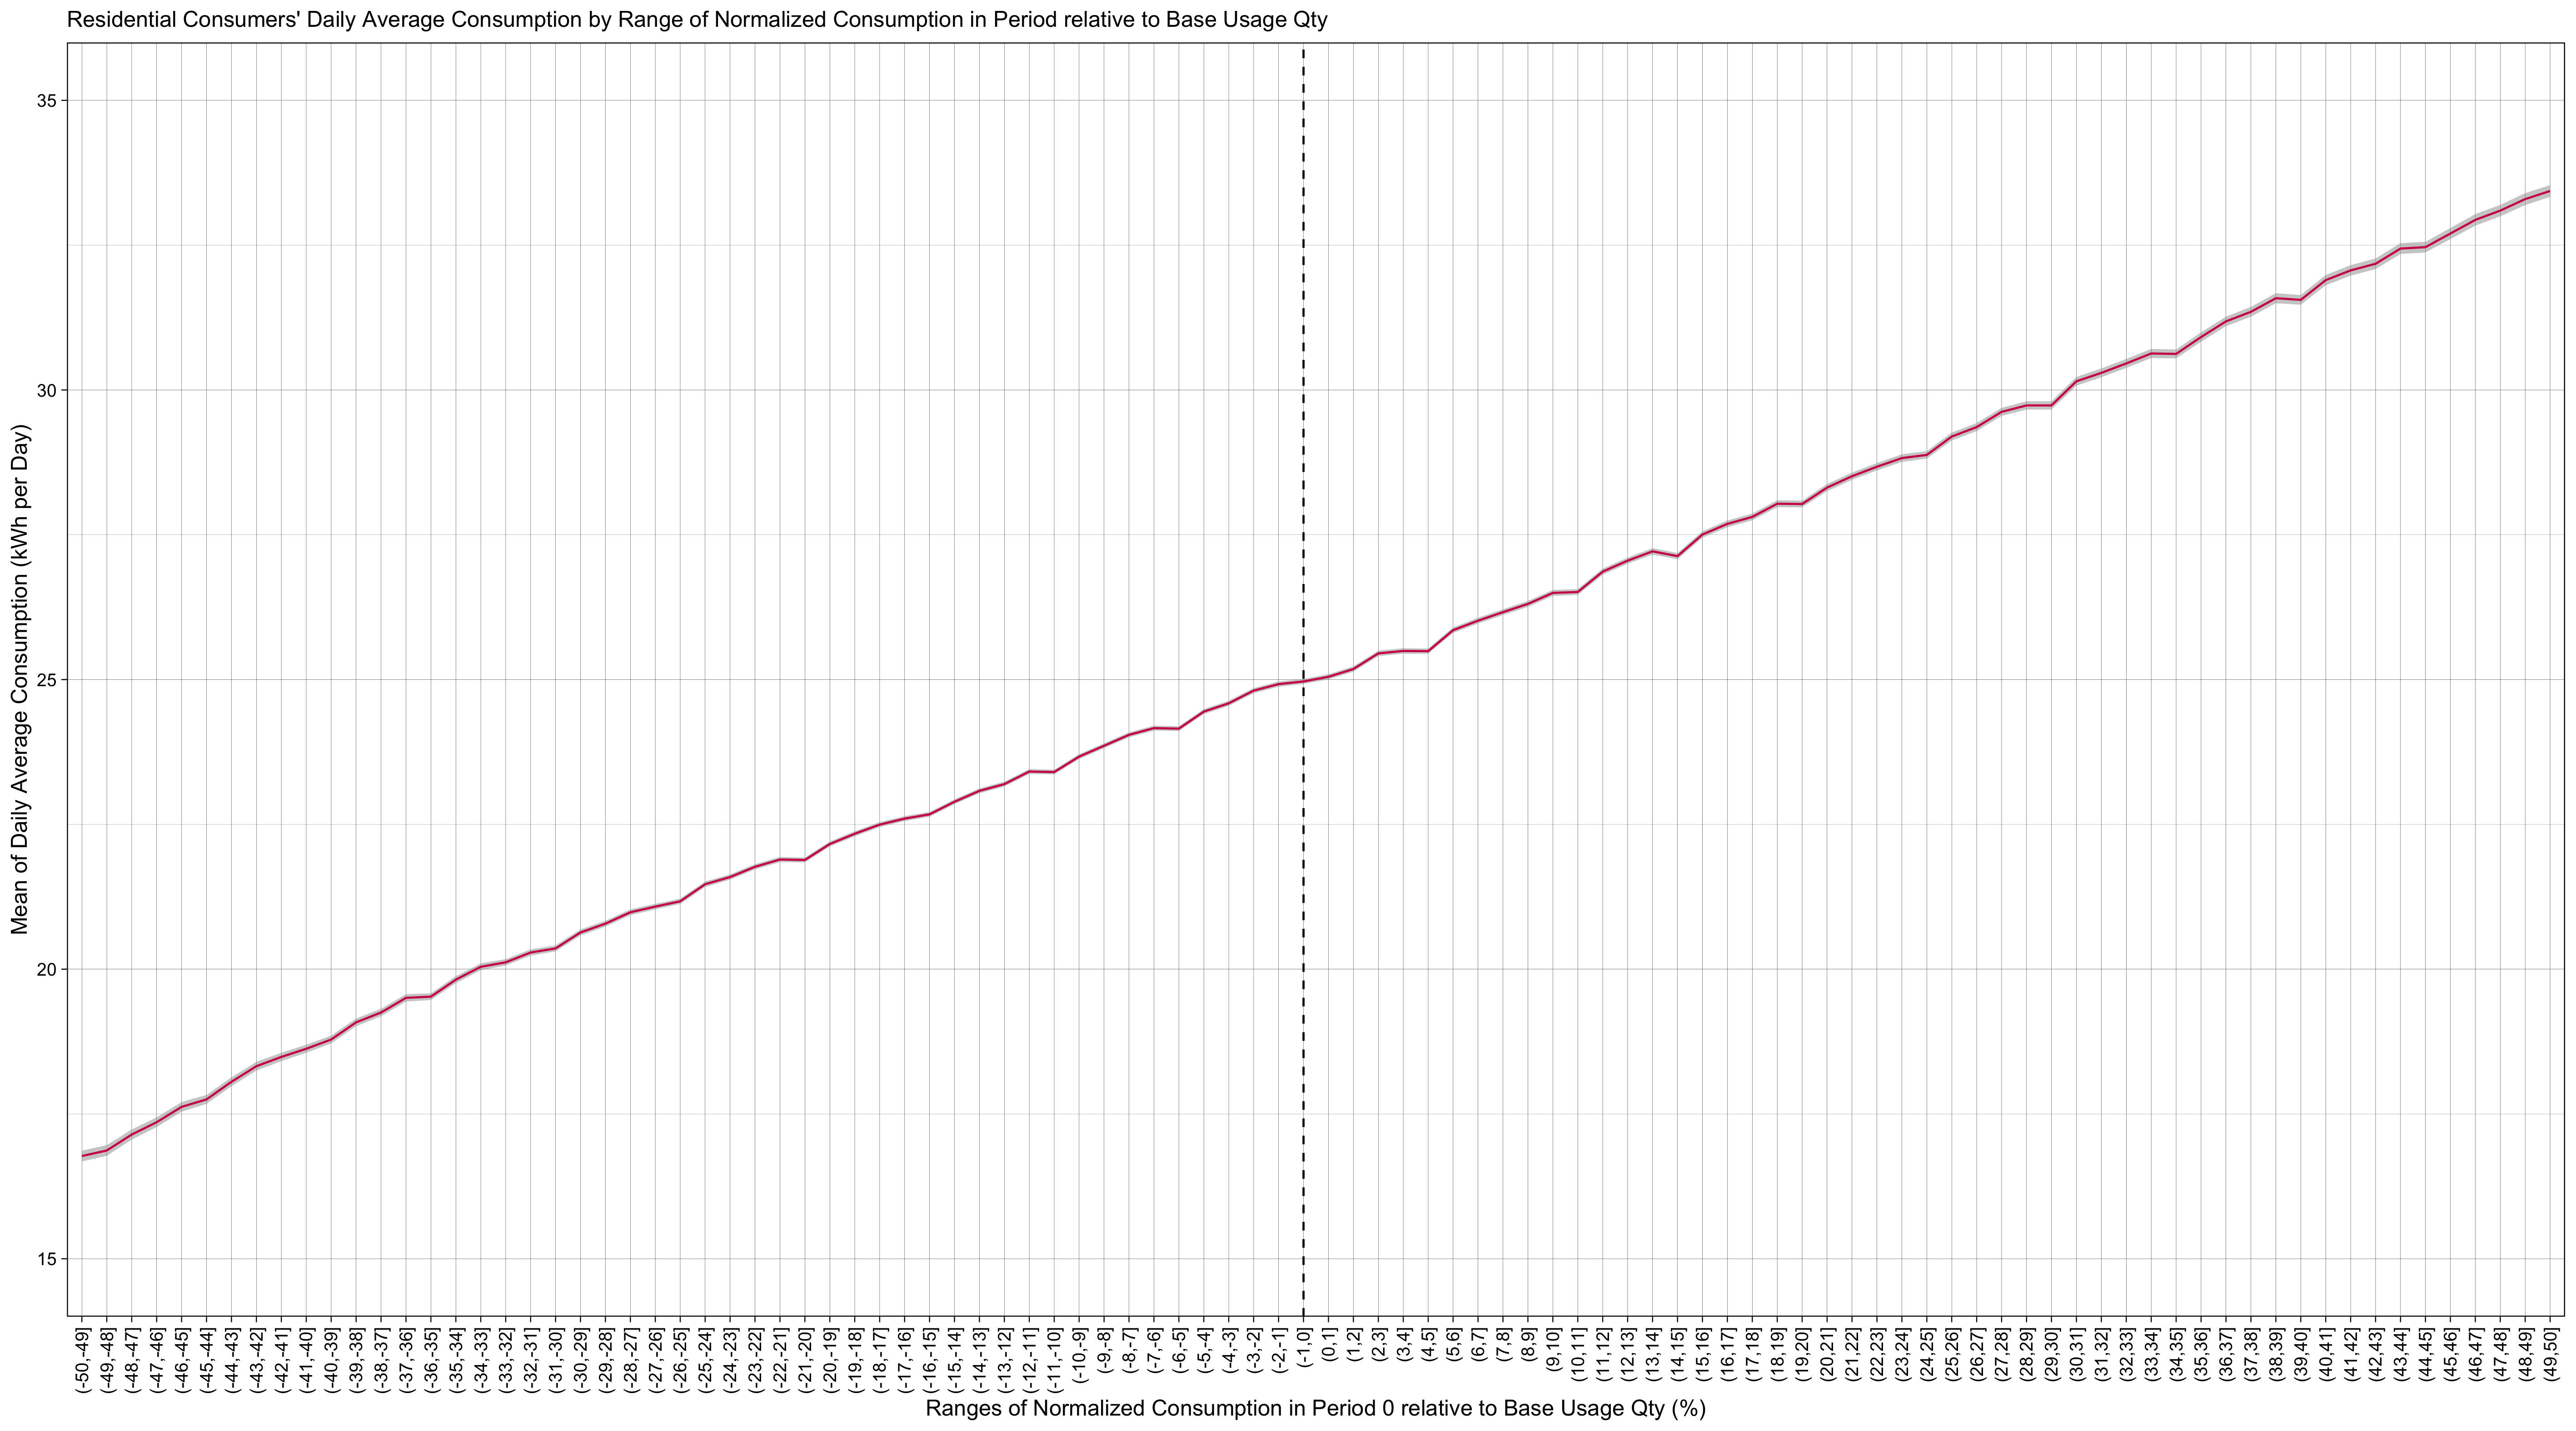
\includegraphics[scale = 0.085]{02_Plots/SMUD-Billing-Data_RD-Approach_Mean-by-Range}
    \caption{Mean of Daily Average Consumption by Ranges of Normalized Consumption in Period 0 (\%)}
%   \subcaption*{\textit{Notes: }}
    \label{Figure:Mean-by-Ranges}
\end{figure}


\clearpage
\begin{figure}
    \centering
    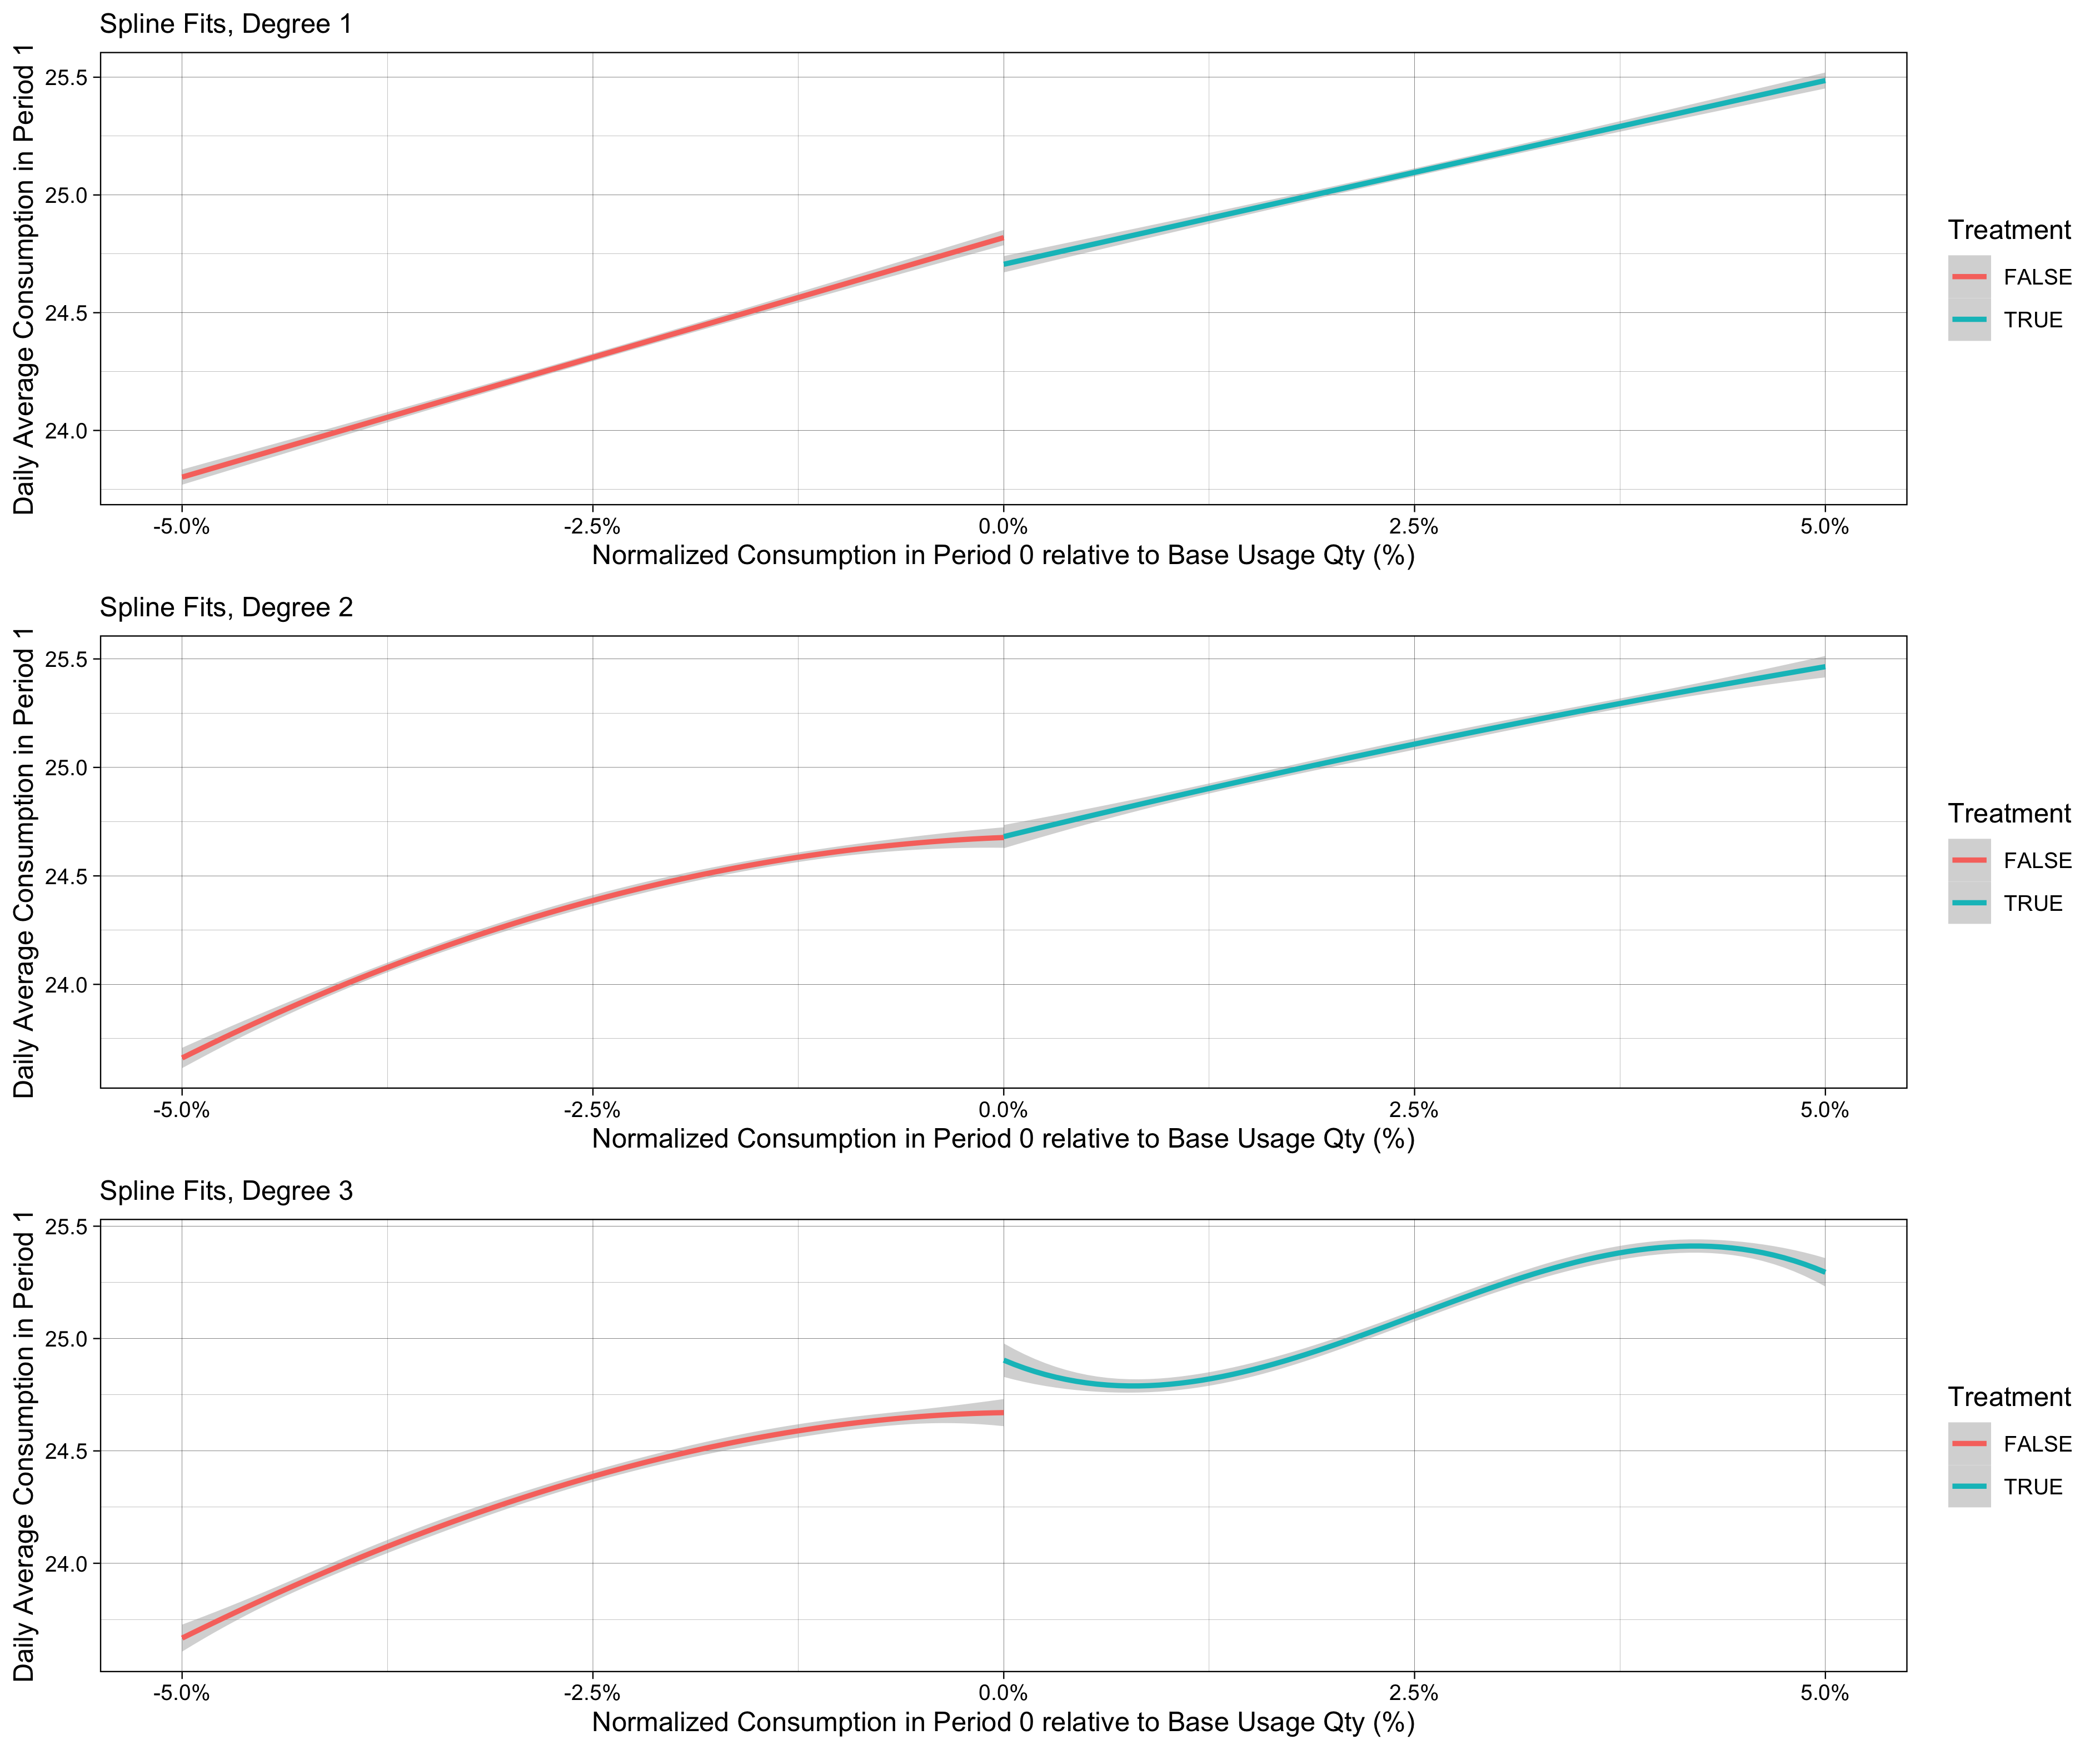
\includegraphics[scale = 0.13]{02_Plots/SMUD-Billing-Data_RD-Approach_Spline_BW-5}
    \caption{Spline Fits - By using Daily Average Consumption in Period 1 with 5\% Bandwidth}
    \label{Figure:Spline_5P}
\end{figure}

\clearpage
\begin{figure}
    \centering
    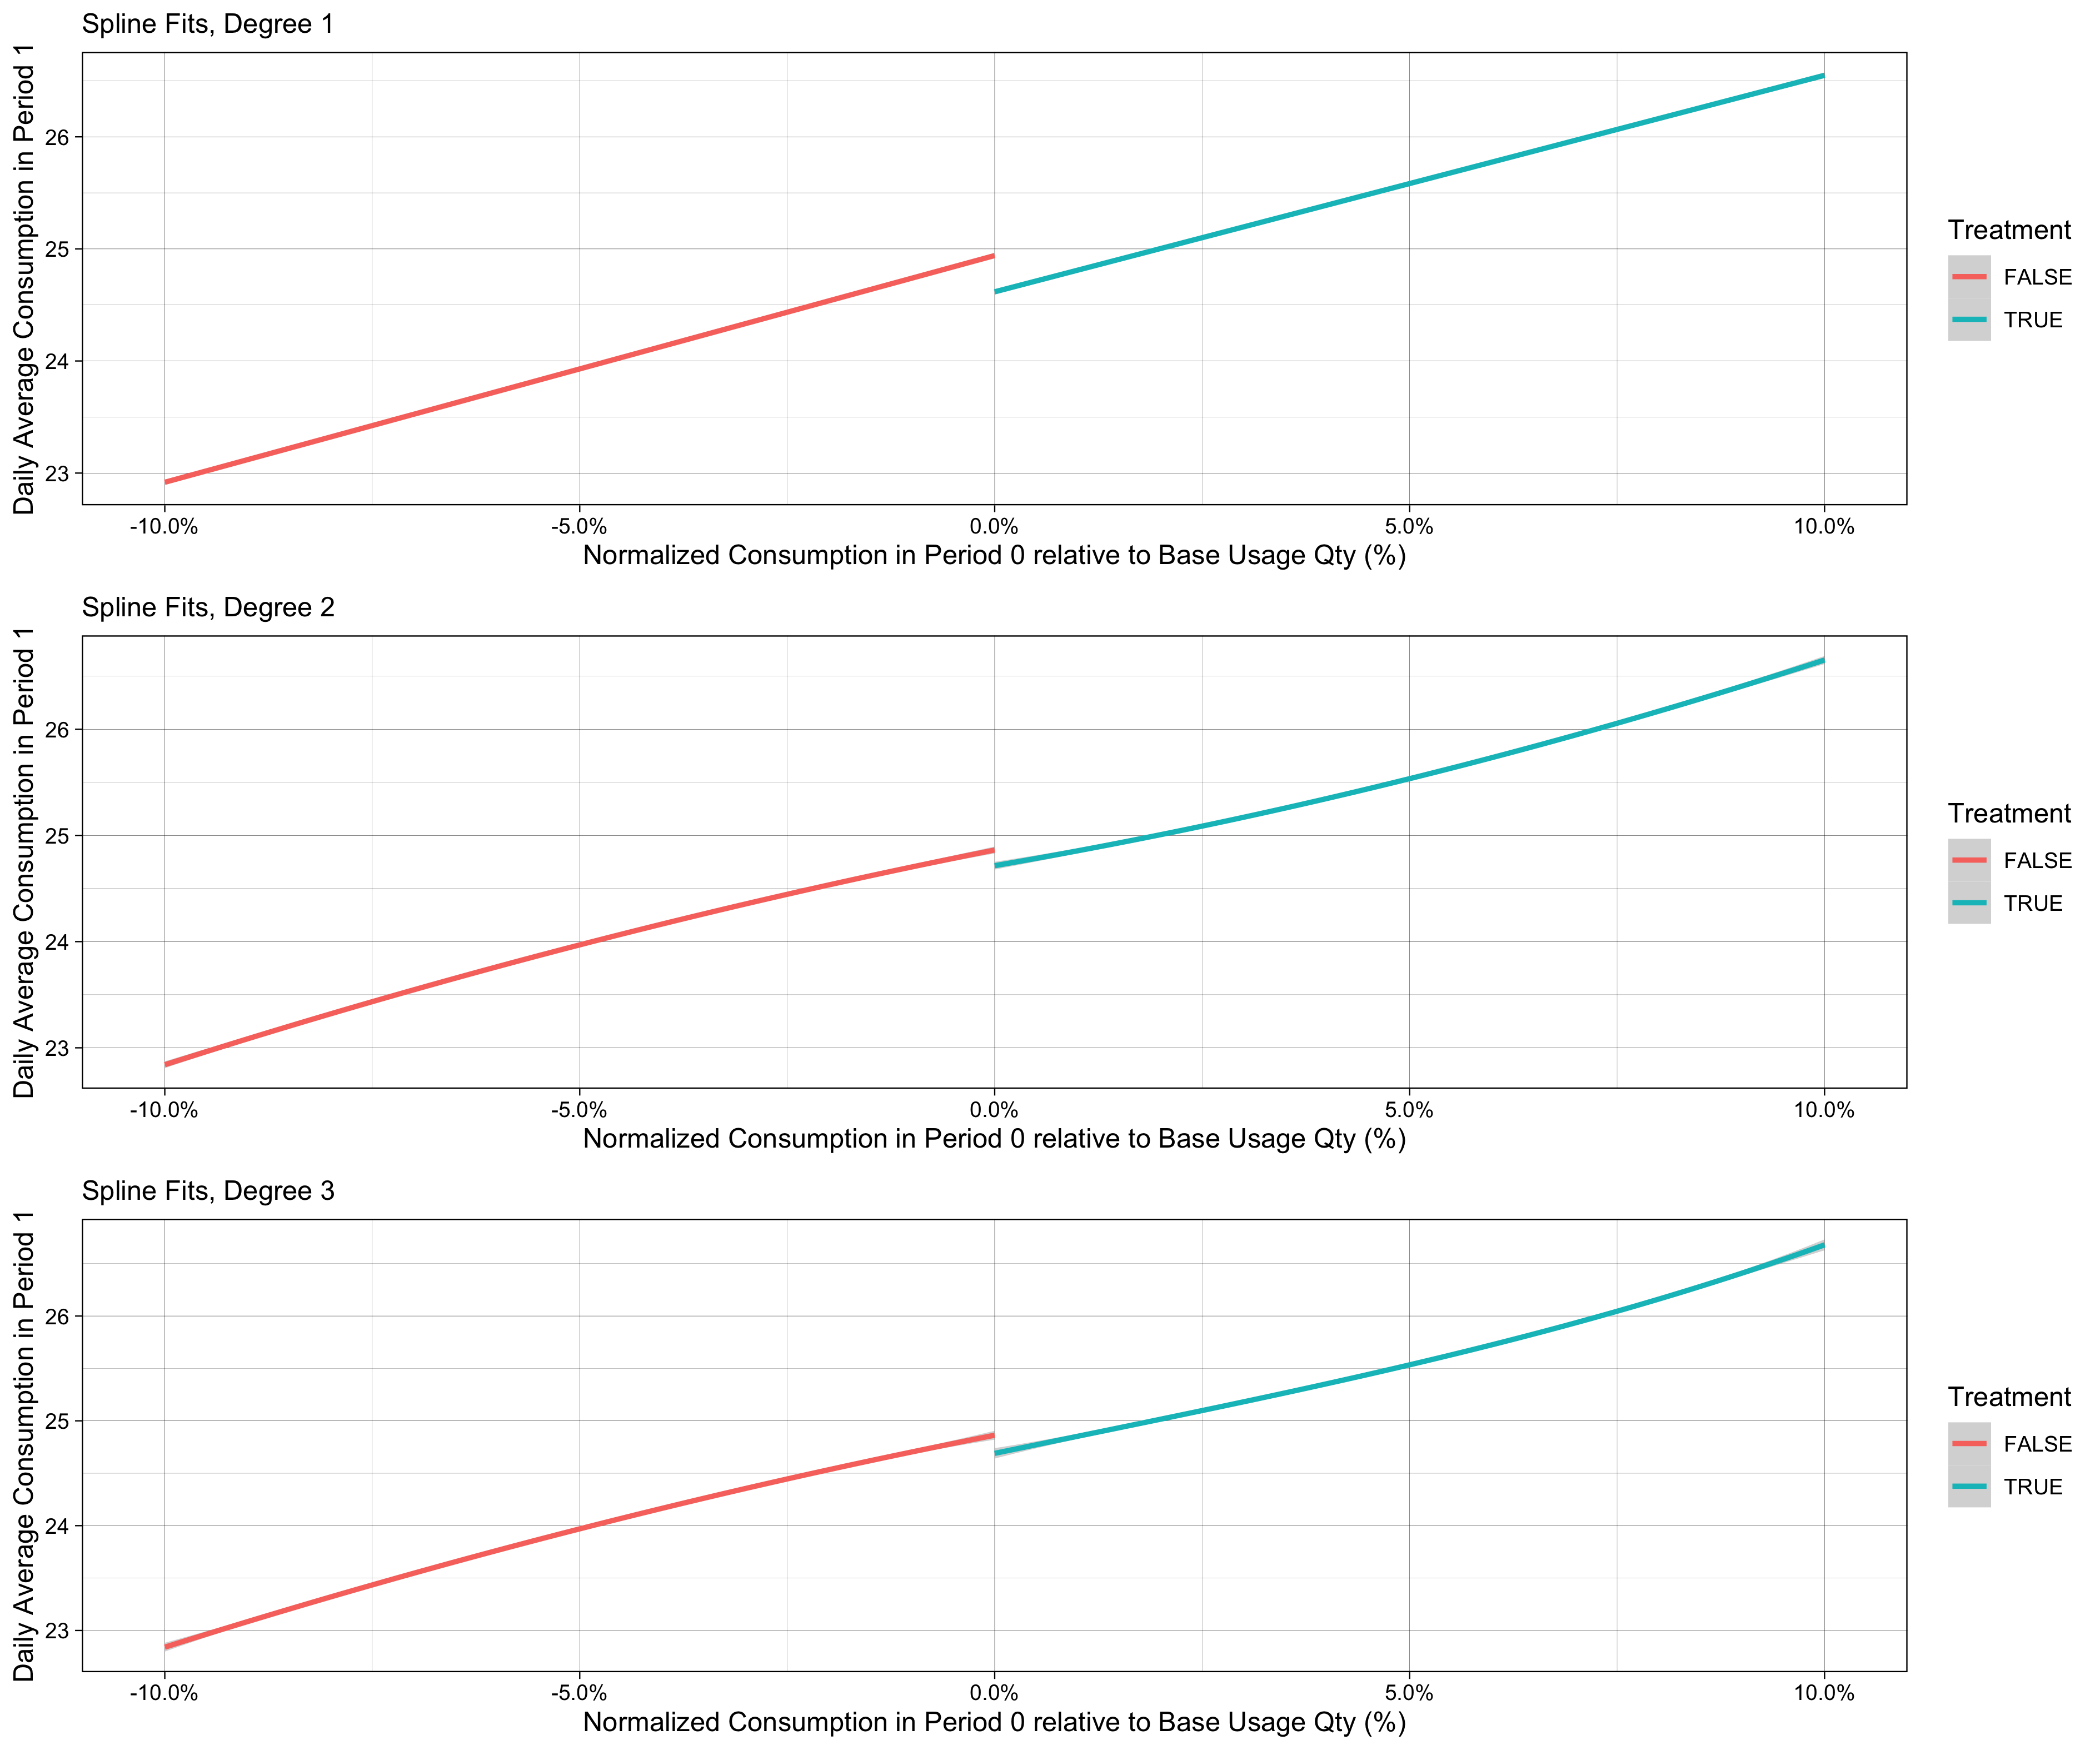
\includegraphics[scale = 0.13]{02_Plots/SMUD-Billing-Data_RD-Approach_Spline_BW-10}
    \caption{Spline Fits - By using Daily Average Consumption in Period 1 with 10\% Bandwidth}
    \label{Figure:Spline_10P}
\end{figure}

\clearpage
\begin{figure}
    \centering
    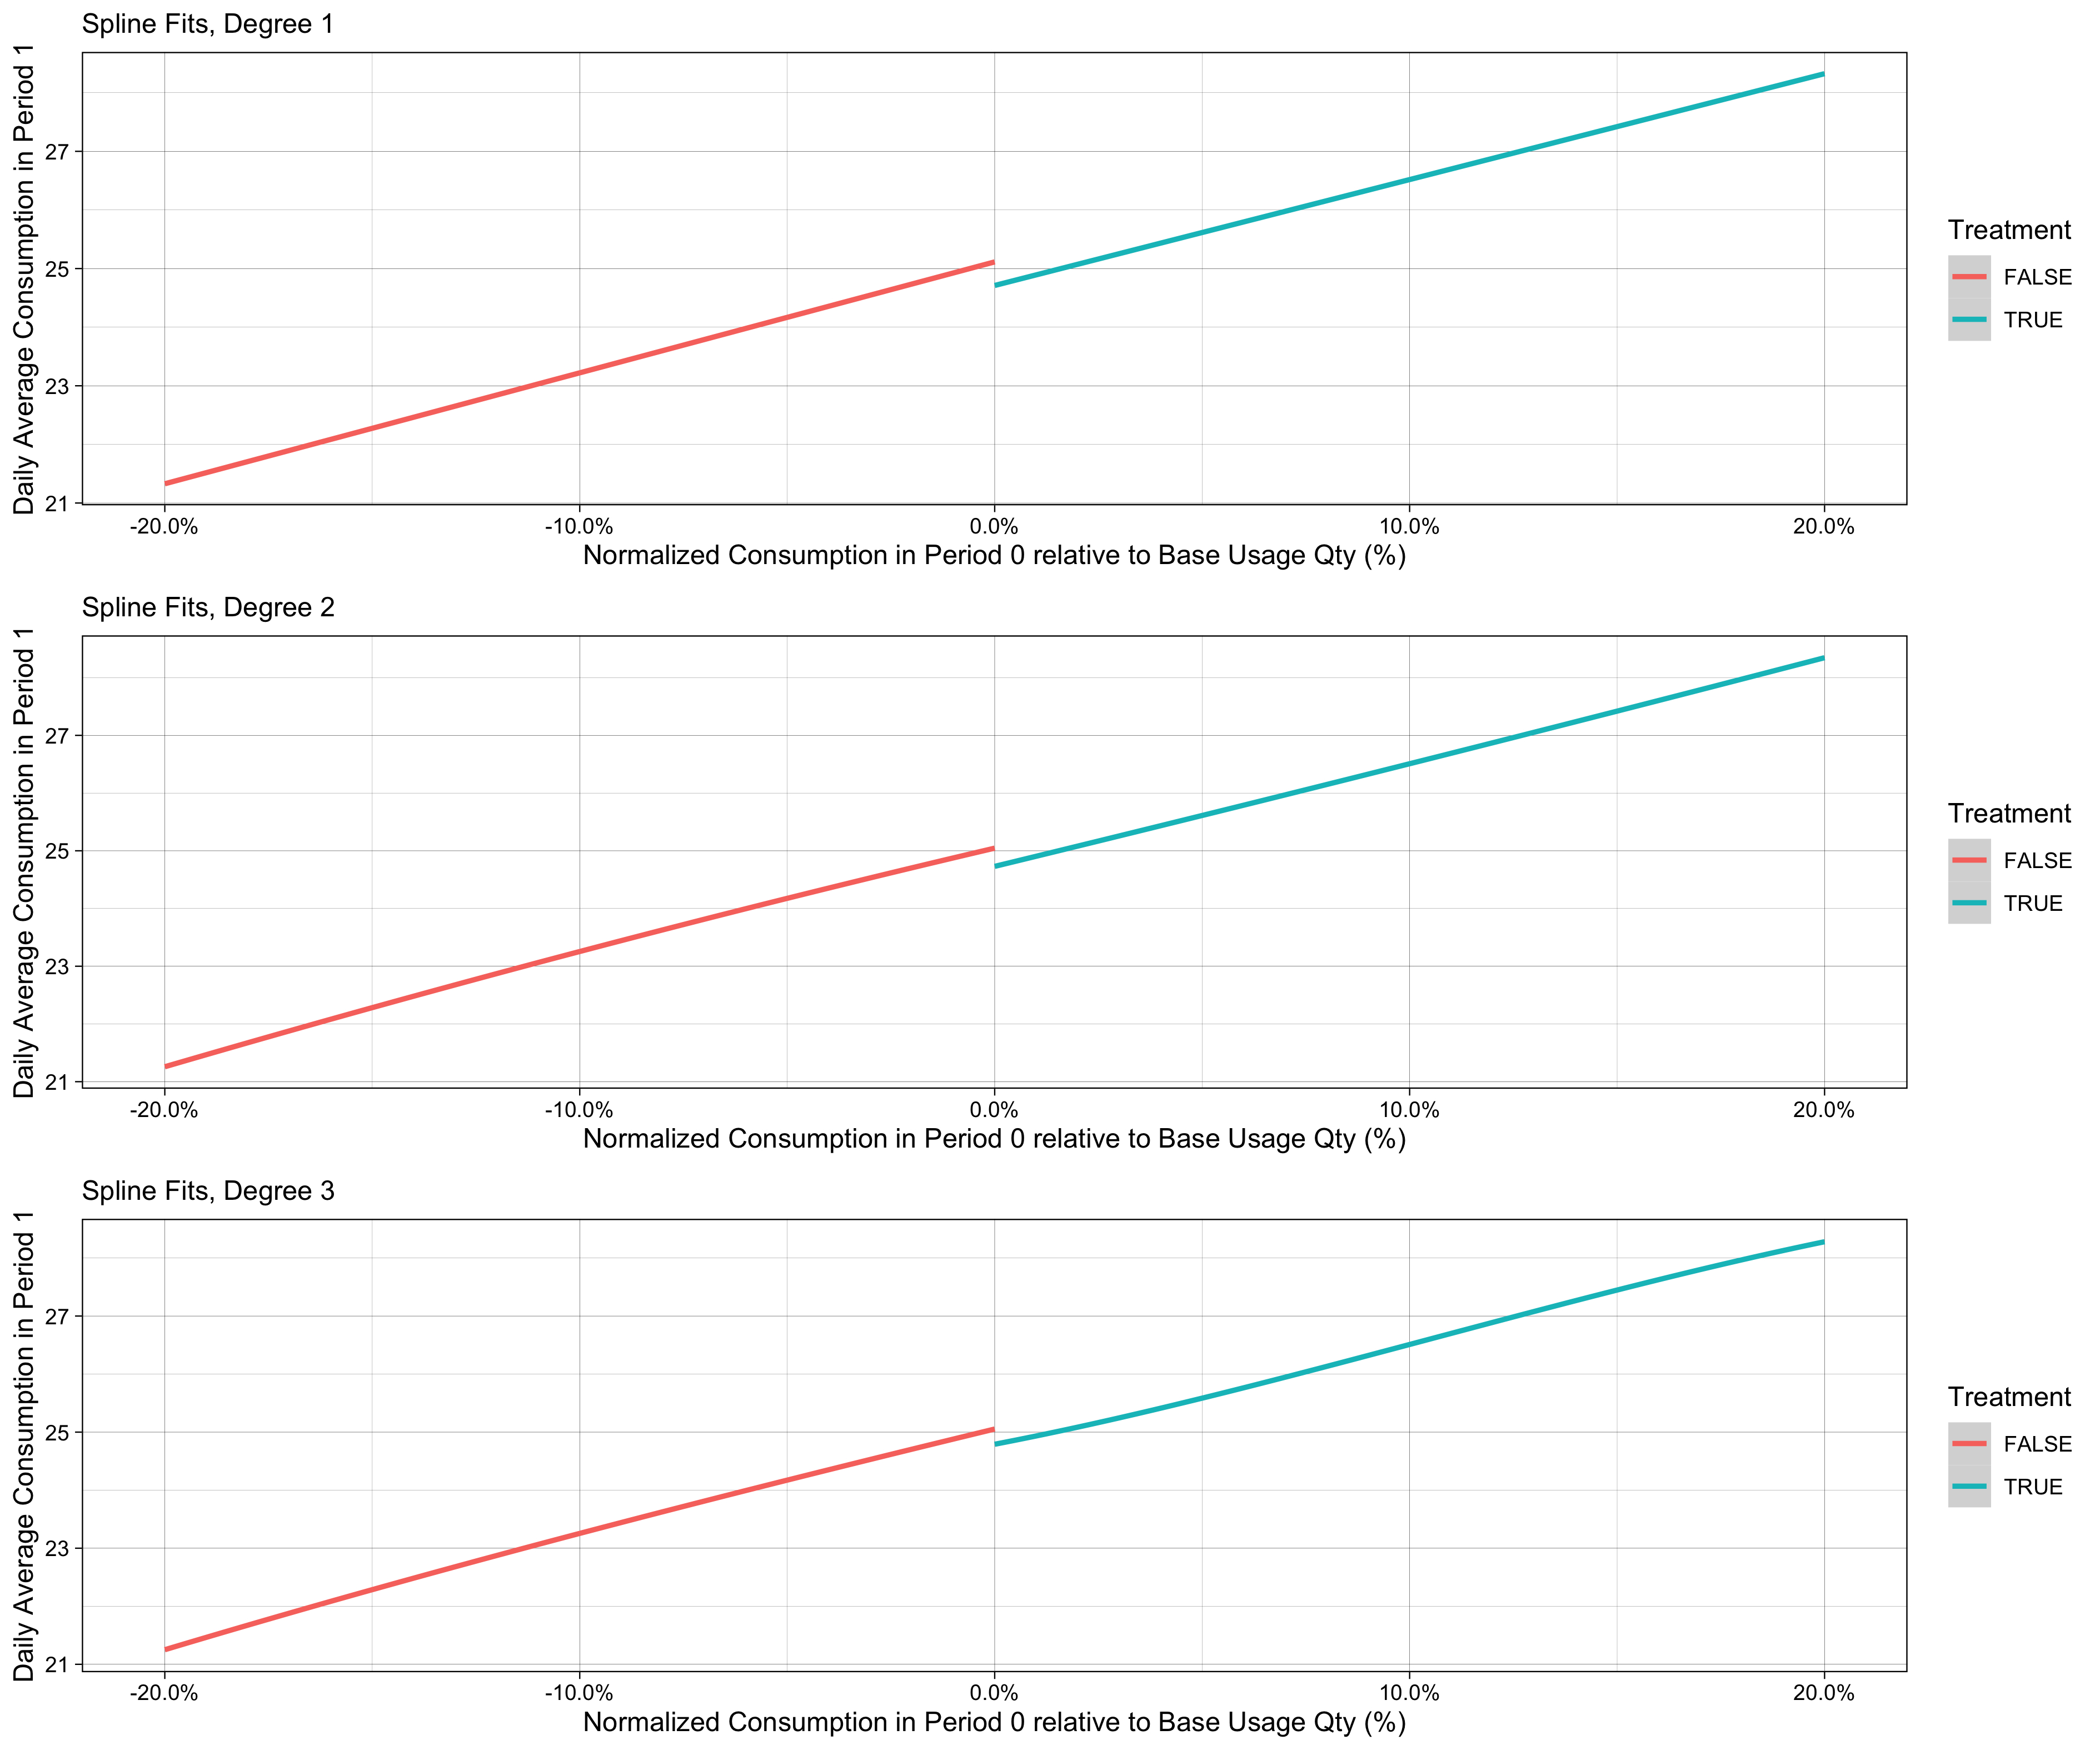
\includegraphics[scale = 0.13]{02_Plots/SMUD-Billing-Data_RD-Approach_Spline_BW-20}
    \caption{Spline Fits - By using Daily Average Consumption in Period 1 with 20\% Bandwidth}
    \label{Figure:Spline_20P}
\end{figure}

\clearpage
\begin{figure}
    \centering
    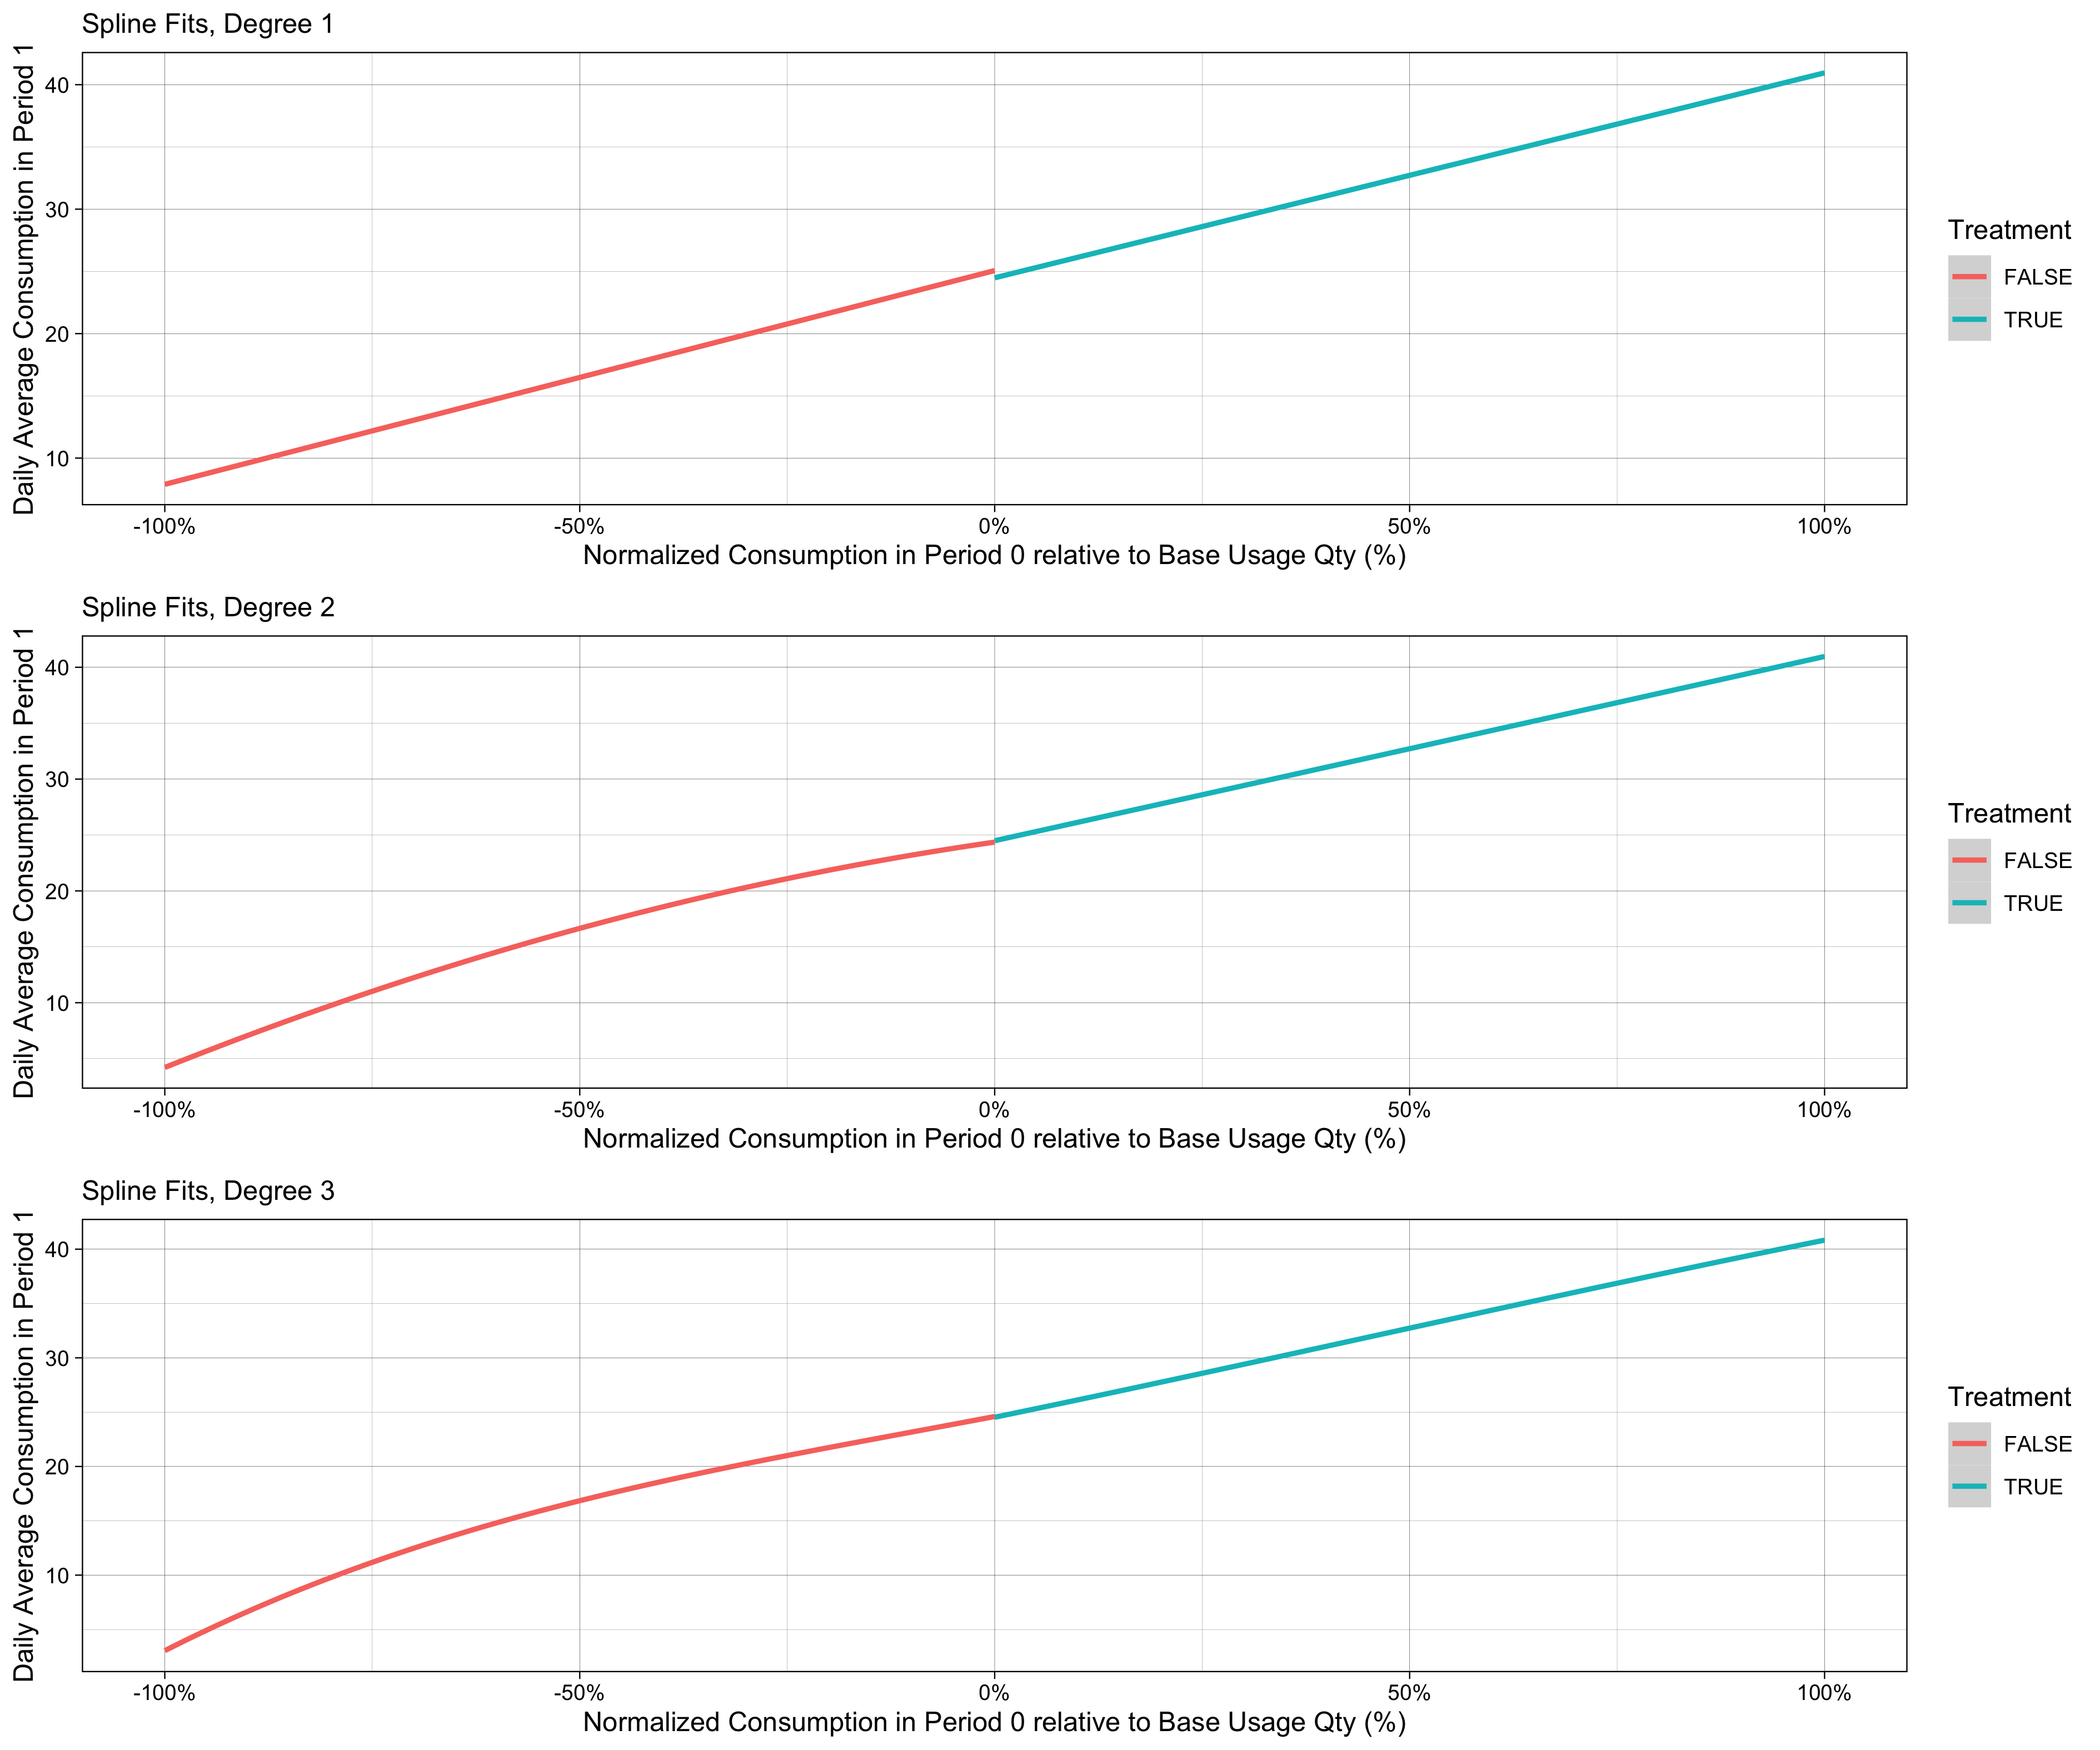
\includegraphics[scale = 0.13]{02_Plots/SMUD-Billing-Data_RD-Approach_Spline_BW-NA}
    \caption{Spline Fits - By using Daily Average Consumption in Period 1}
    \label{Figure:Spline_NA}
\end{figure}


\clearpage
\begin{figure}
    \centering
    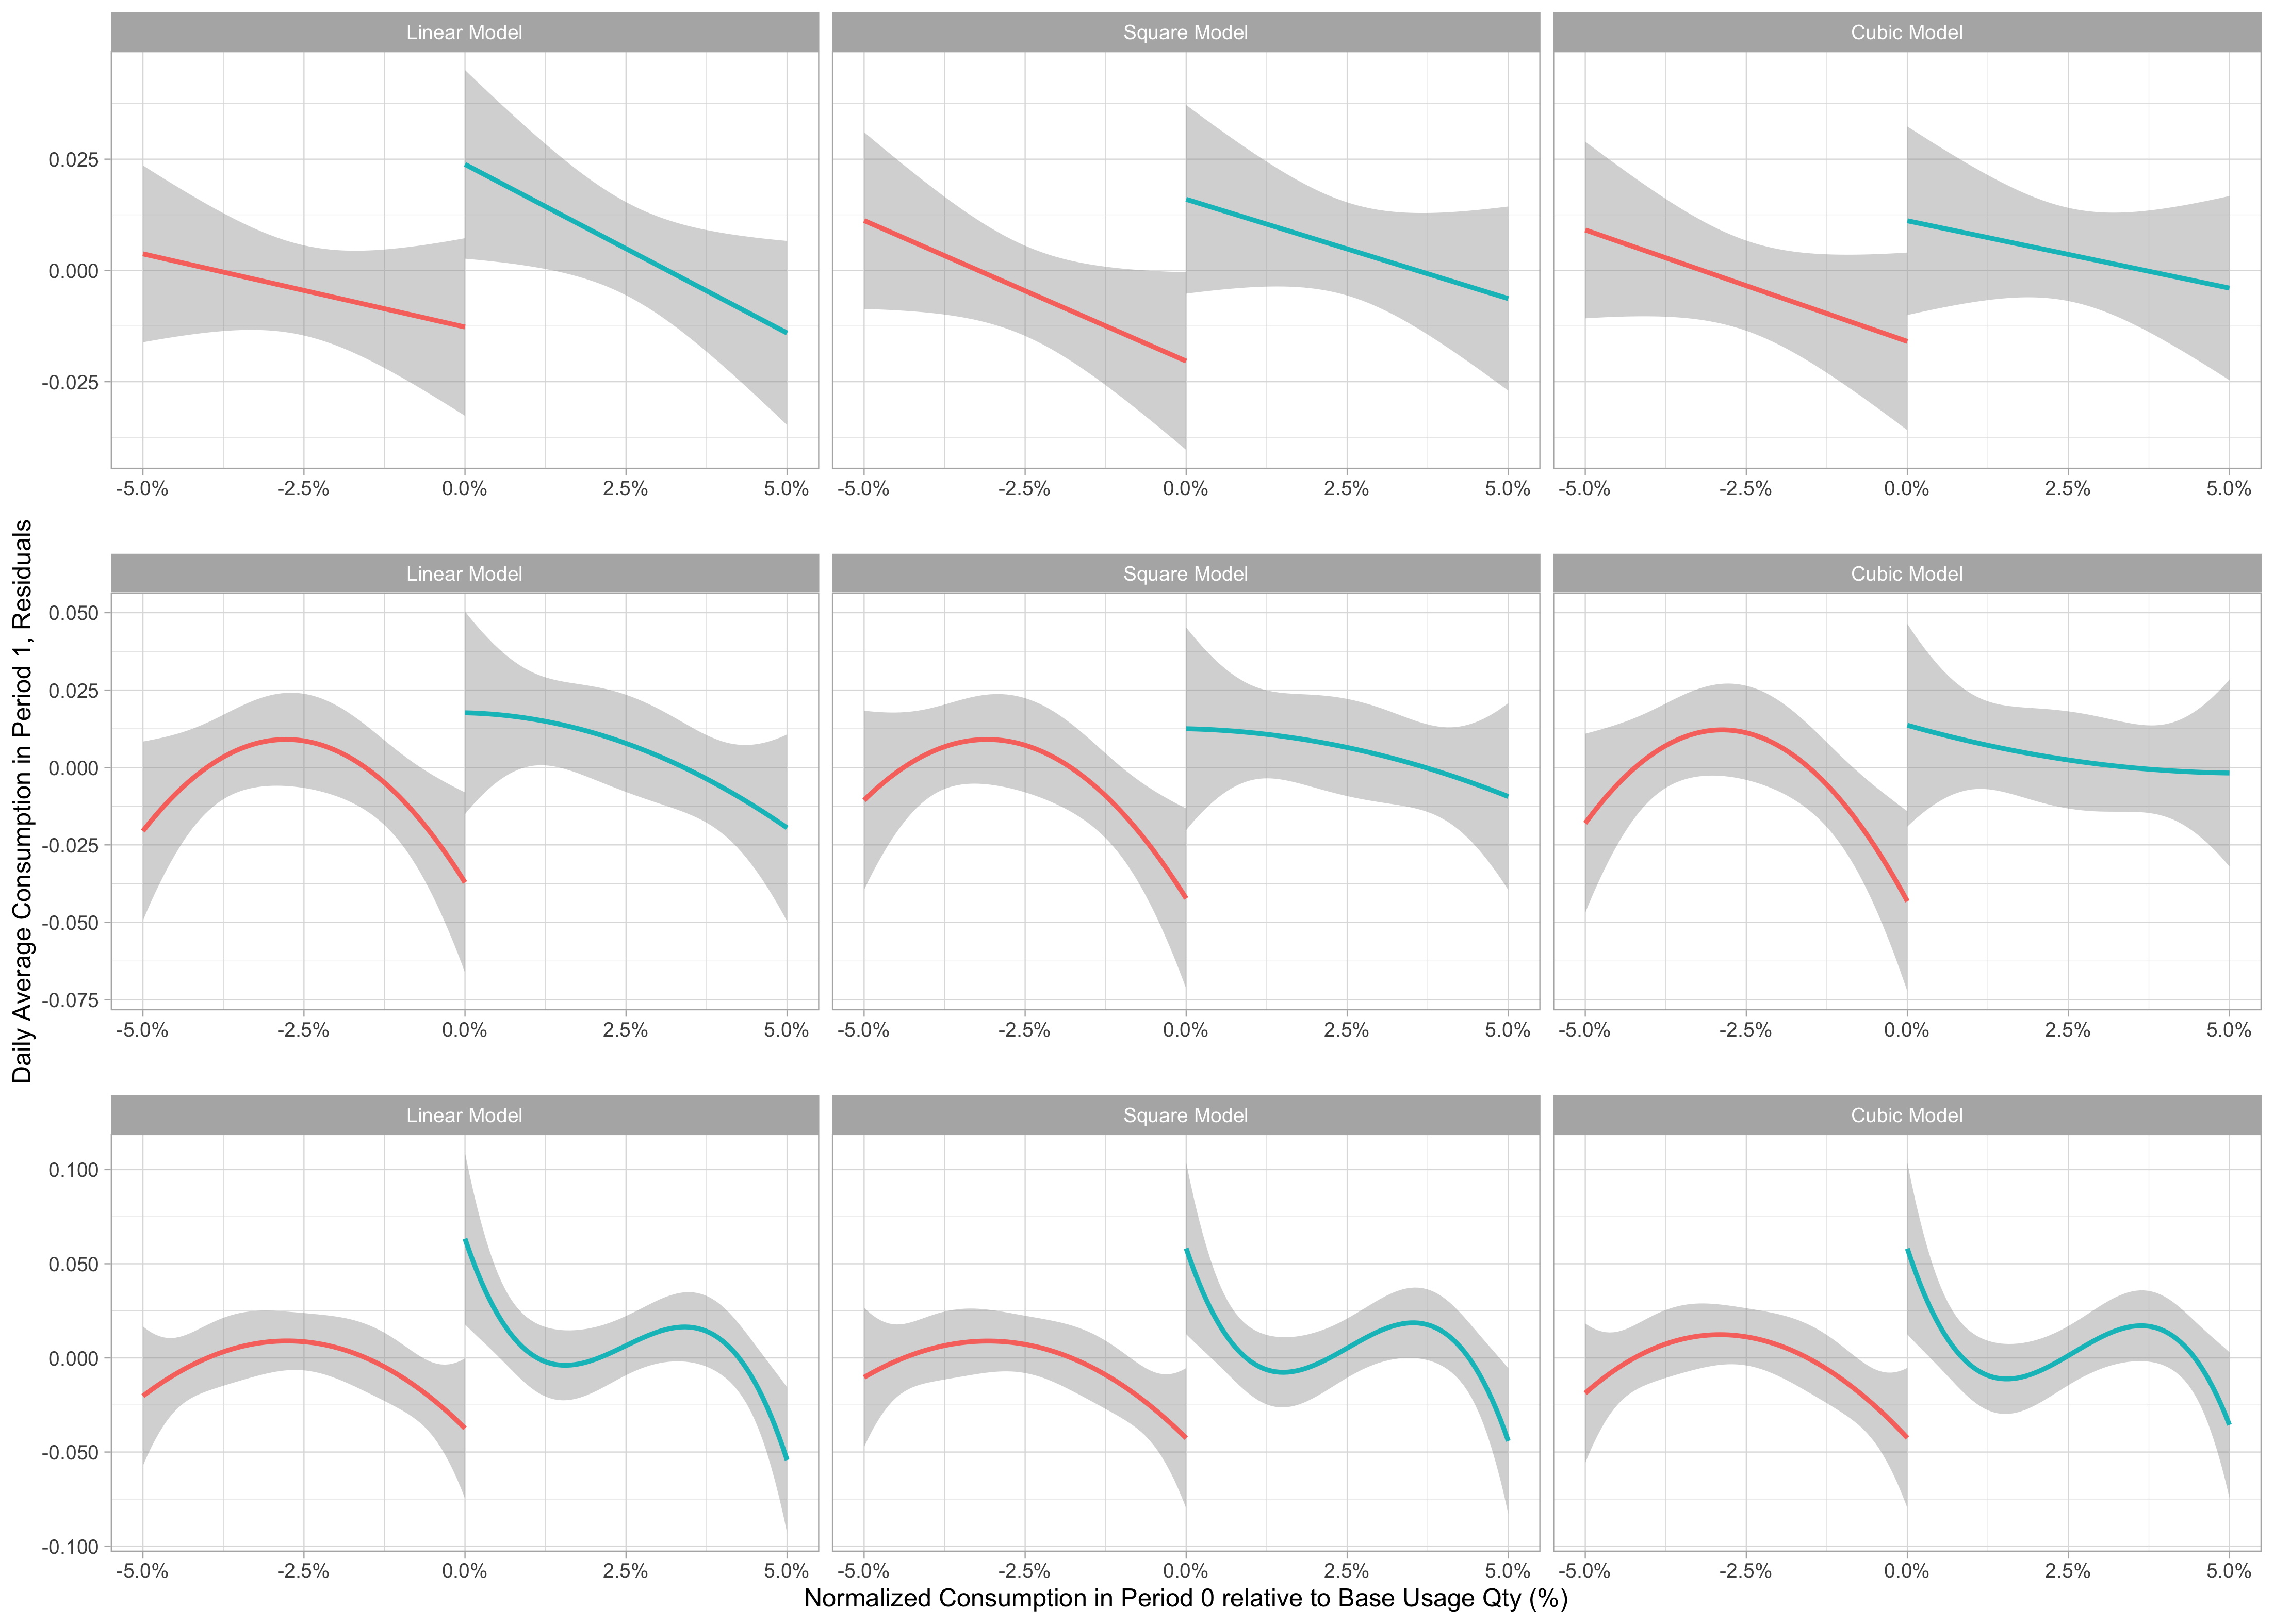
\includegraphics[scale = 0.085]{02_Plots/SMUD-Billing-Data_RD-Approach_Residuals_BW-5}
    \caption{Spline Fits - By using Residuals with 5\% Bandwidth}
    \label{Figure:Residuals_5P}
\end{figure}

\begin{figure}
    \centering
    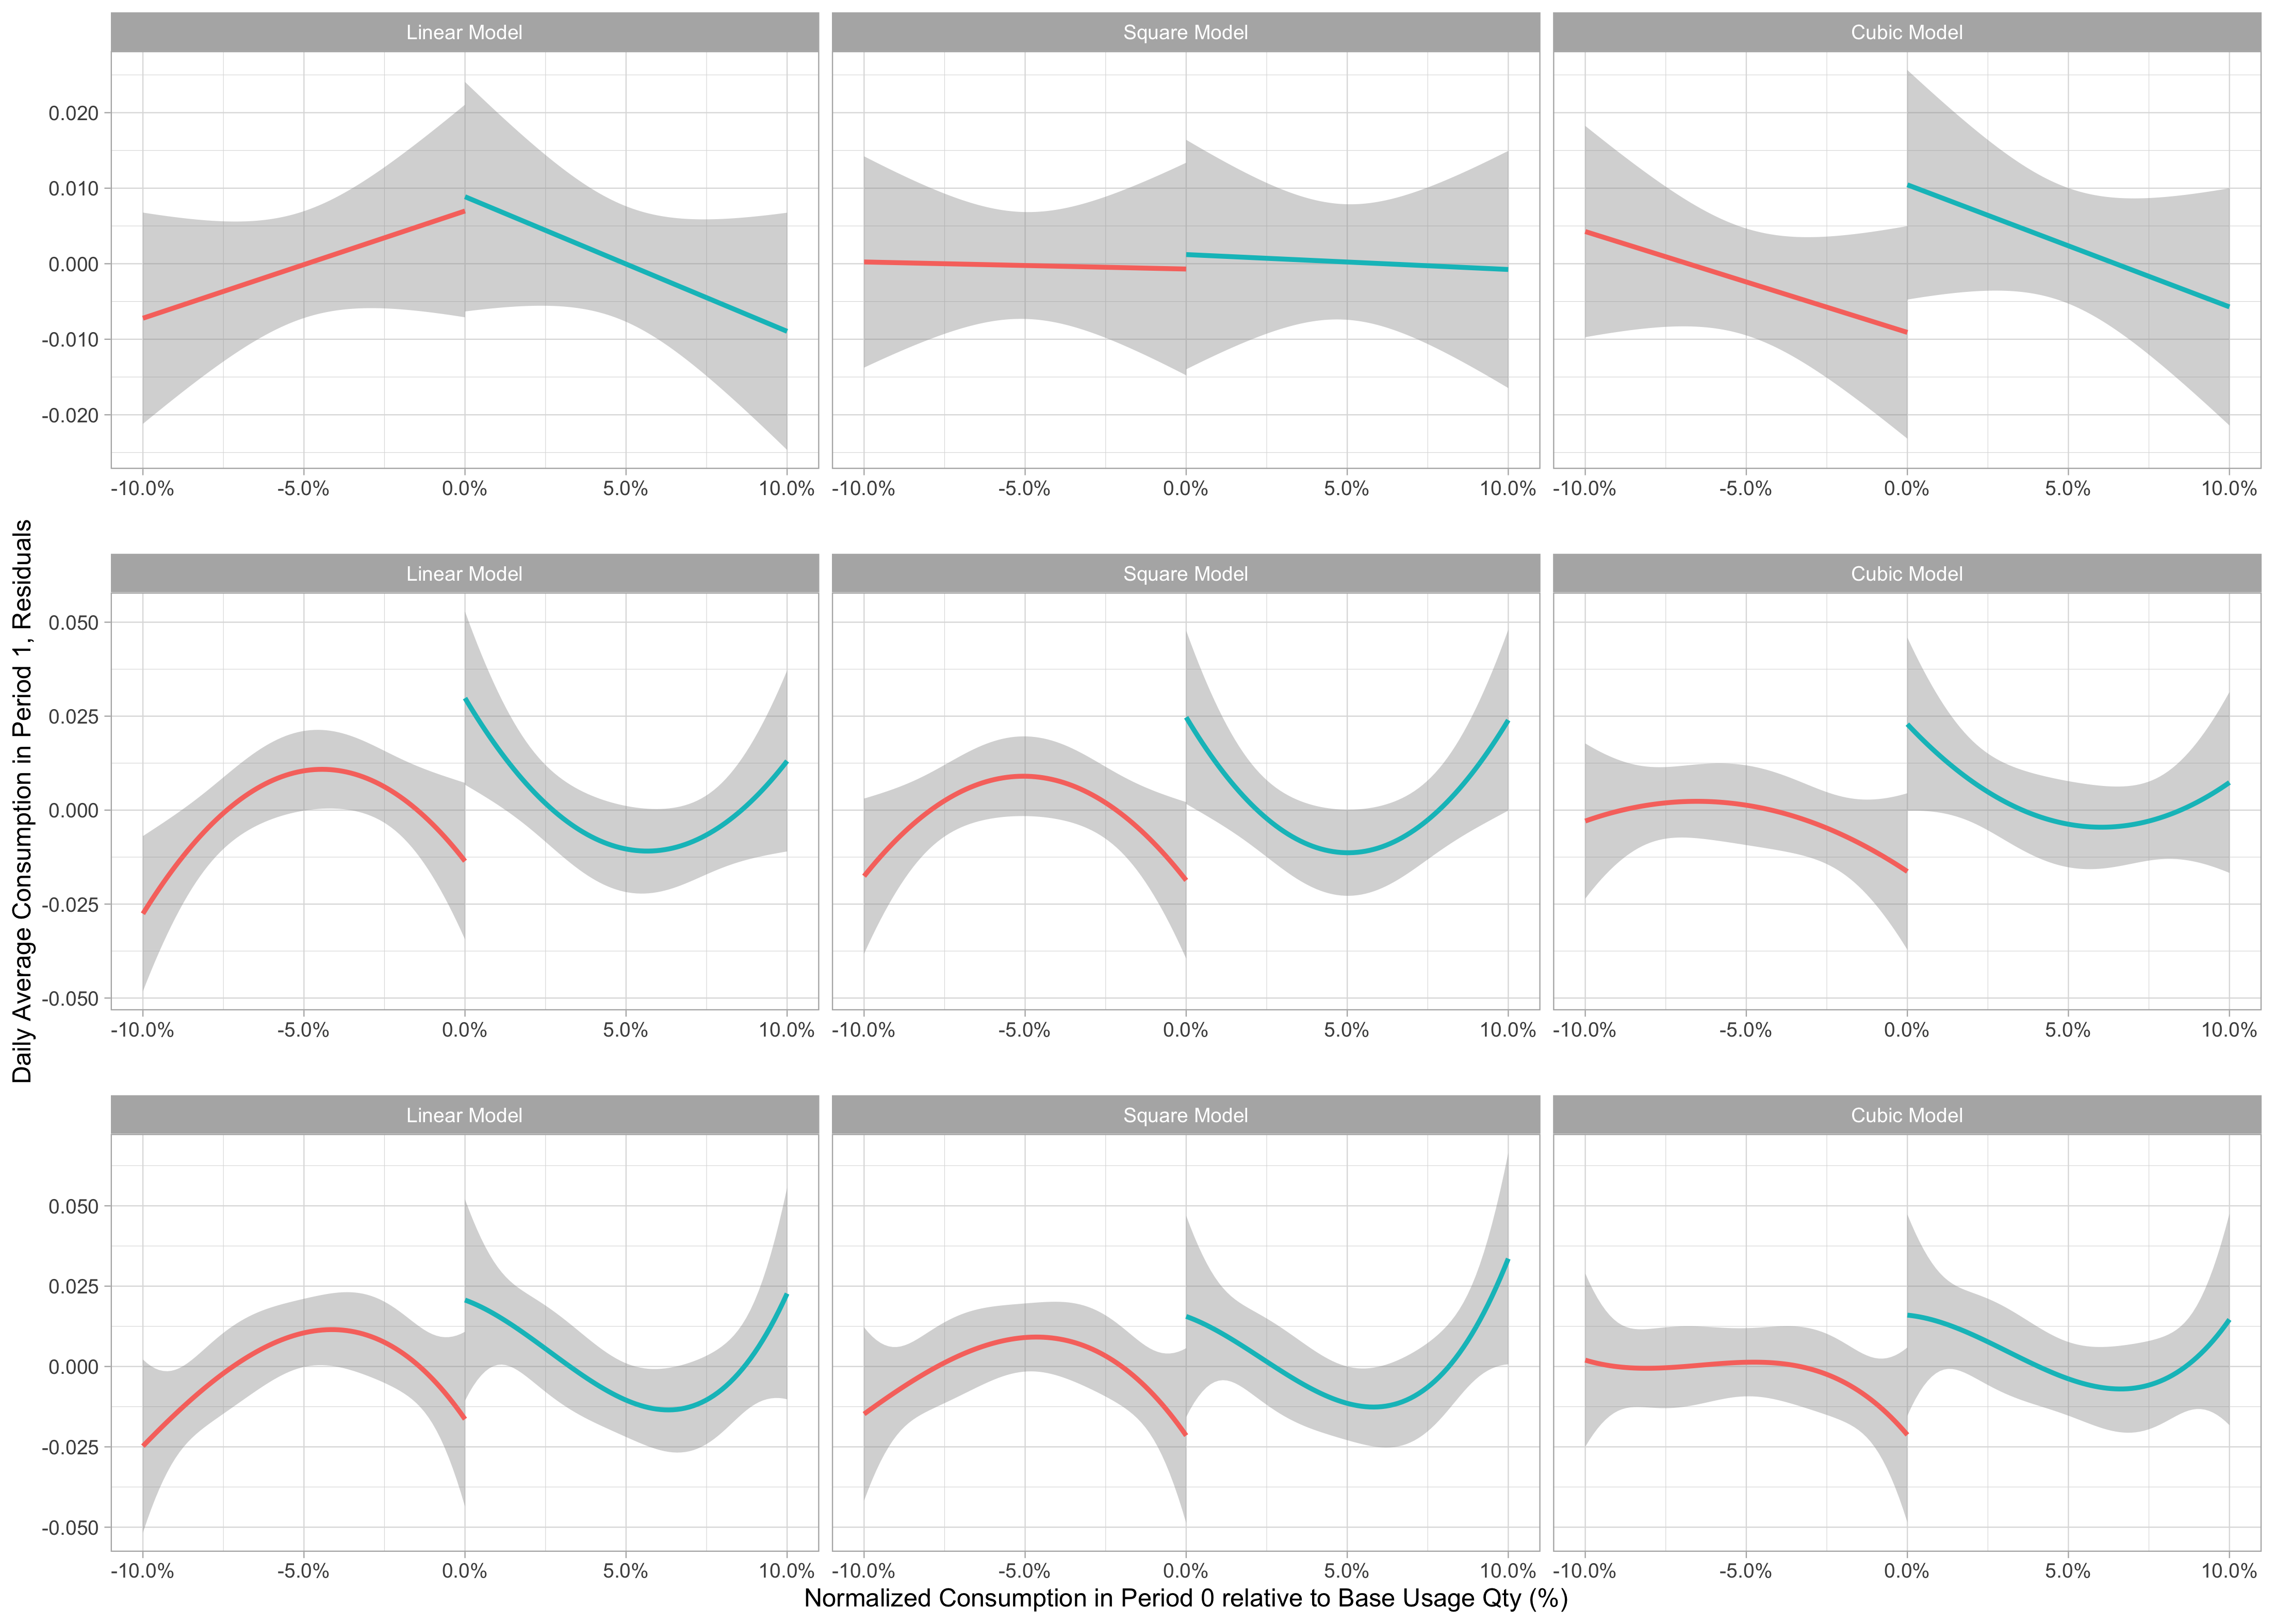
\includegraphics[scale = 0.085]{02_Plots/SMUD-Billing-Data_RD-Approach_Residuals_BW-10}
    \caption{Spline Fits - By using Residuals with 10\% Bandwidth}
    \label{Figure:Residuals_10P}
\end{figure}

\clearpage
\begin{figure}
    \centering
    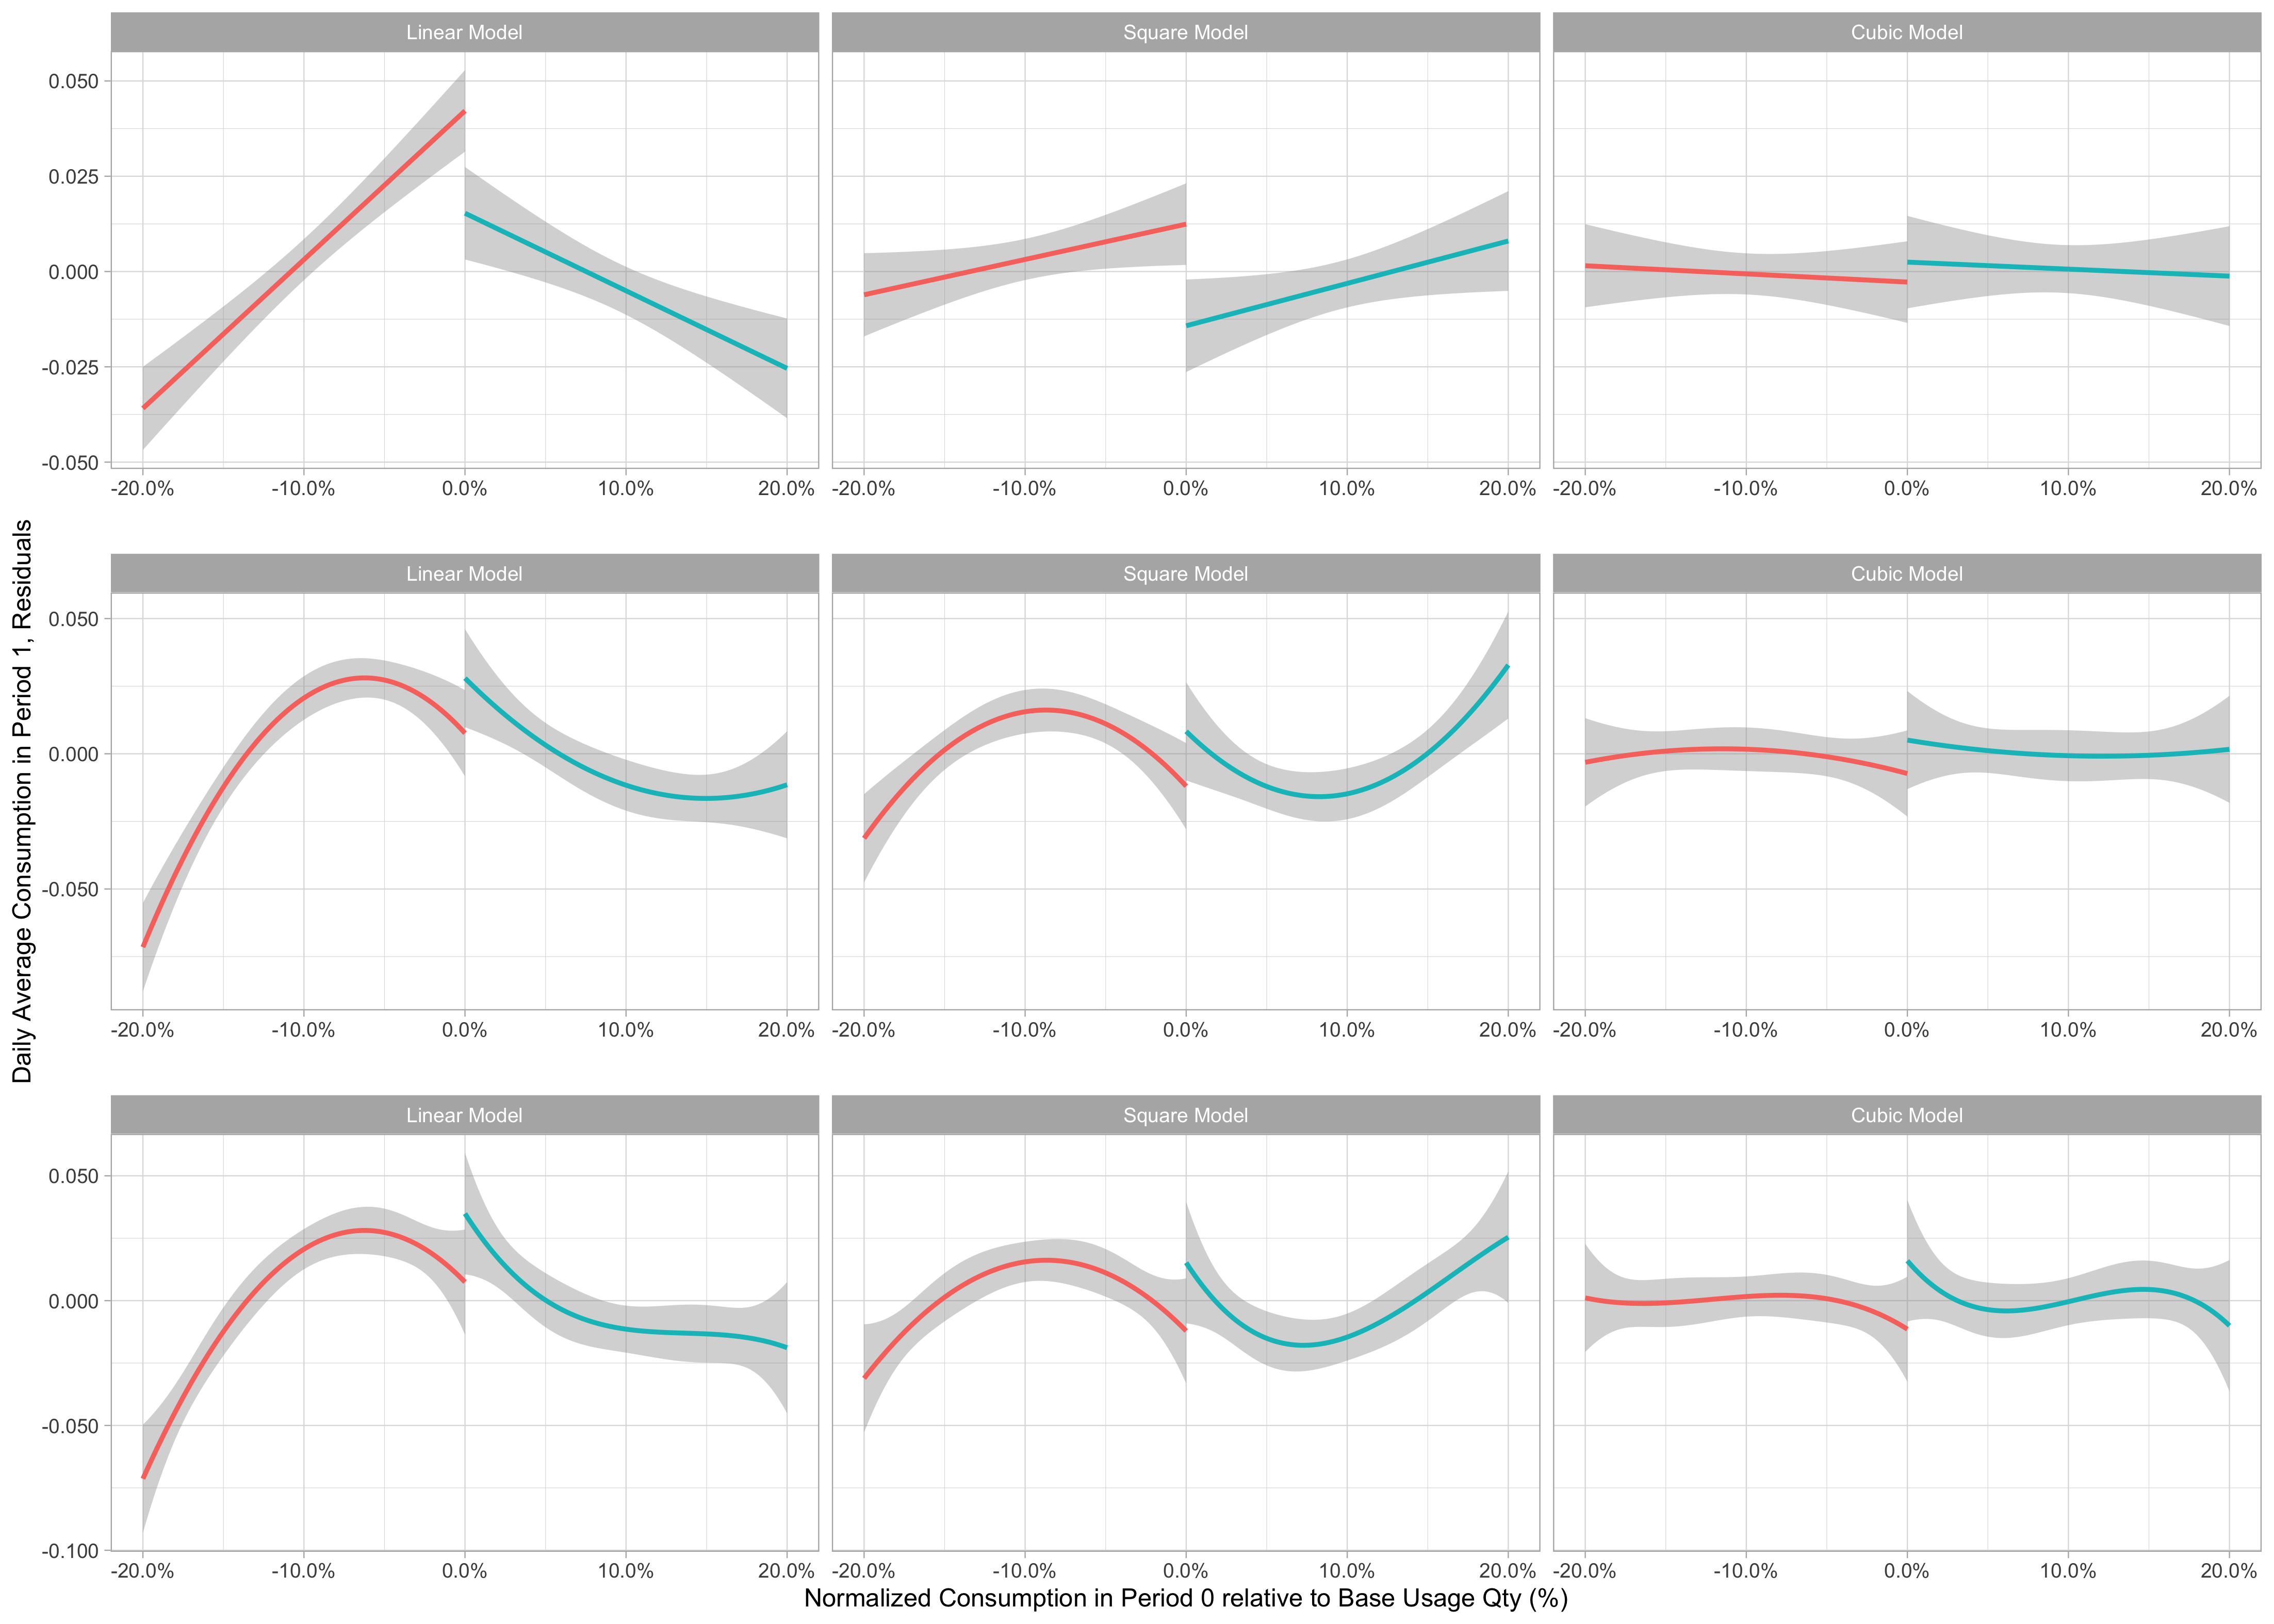
\includegraphics[scale = 0.085]{02_Plots/SMUD-Billing-Data_RD-Approach_Residuals_BW-20}
    \caption{Spline Fits - By using Residuals with 20\% Bandwidth}
    \label{Figure:Residuals_20P}
\end{figure}

\begin{figure}
    \centering
    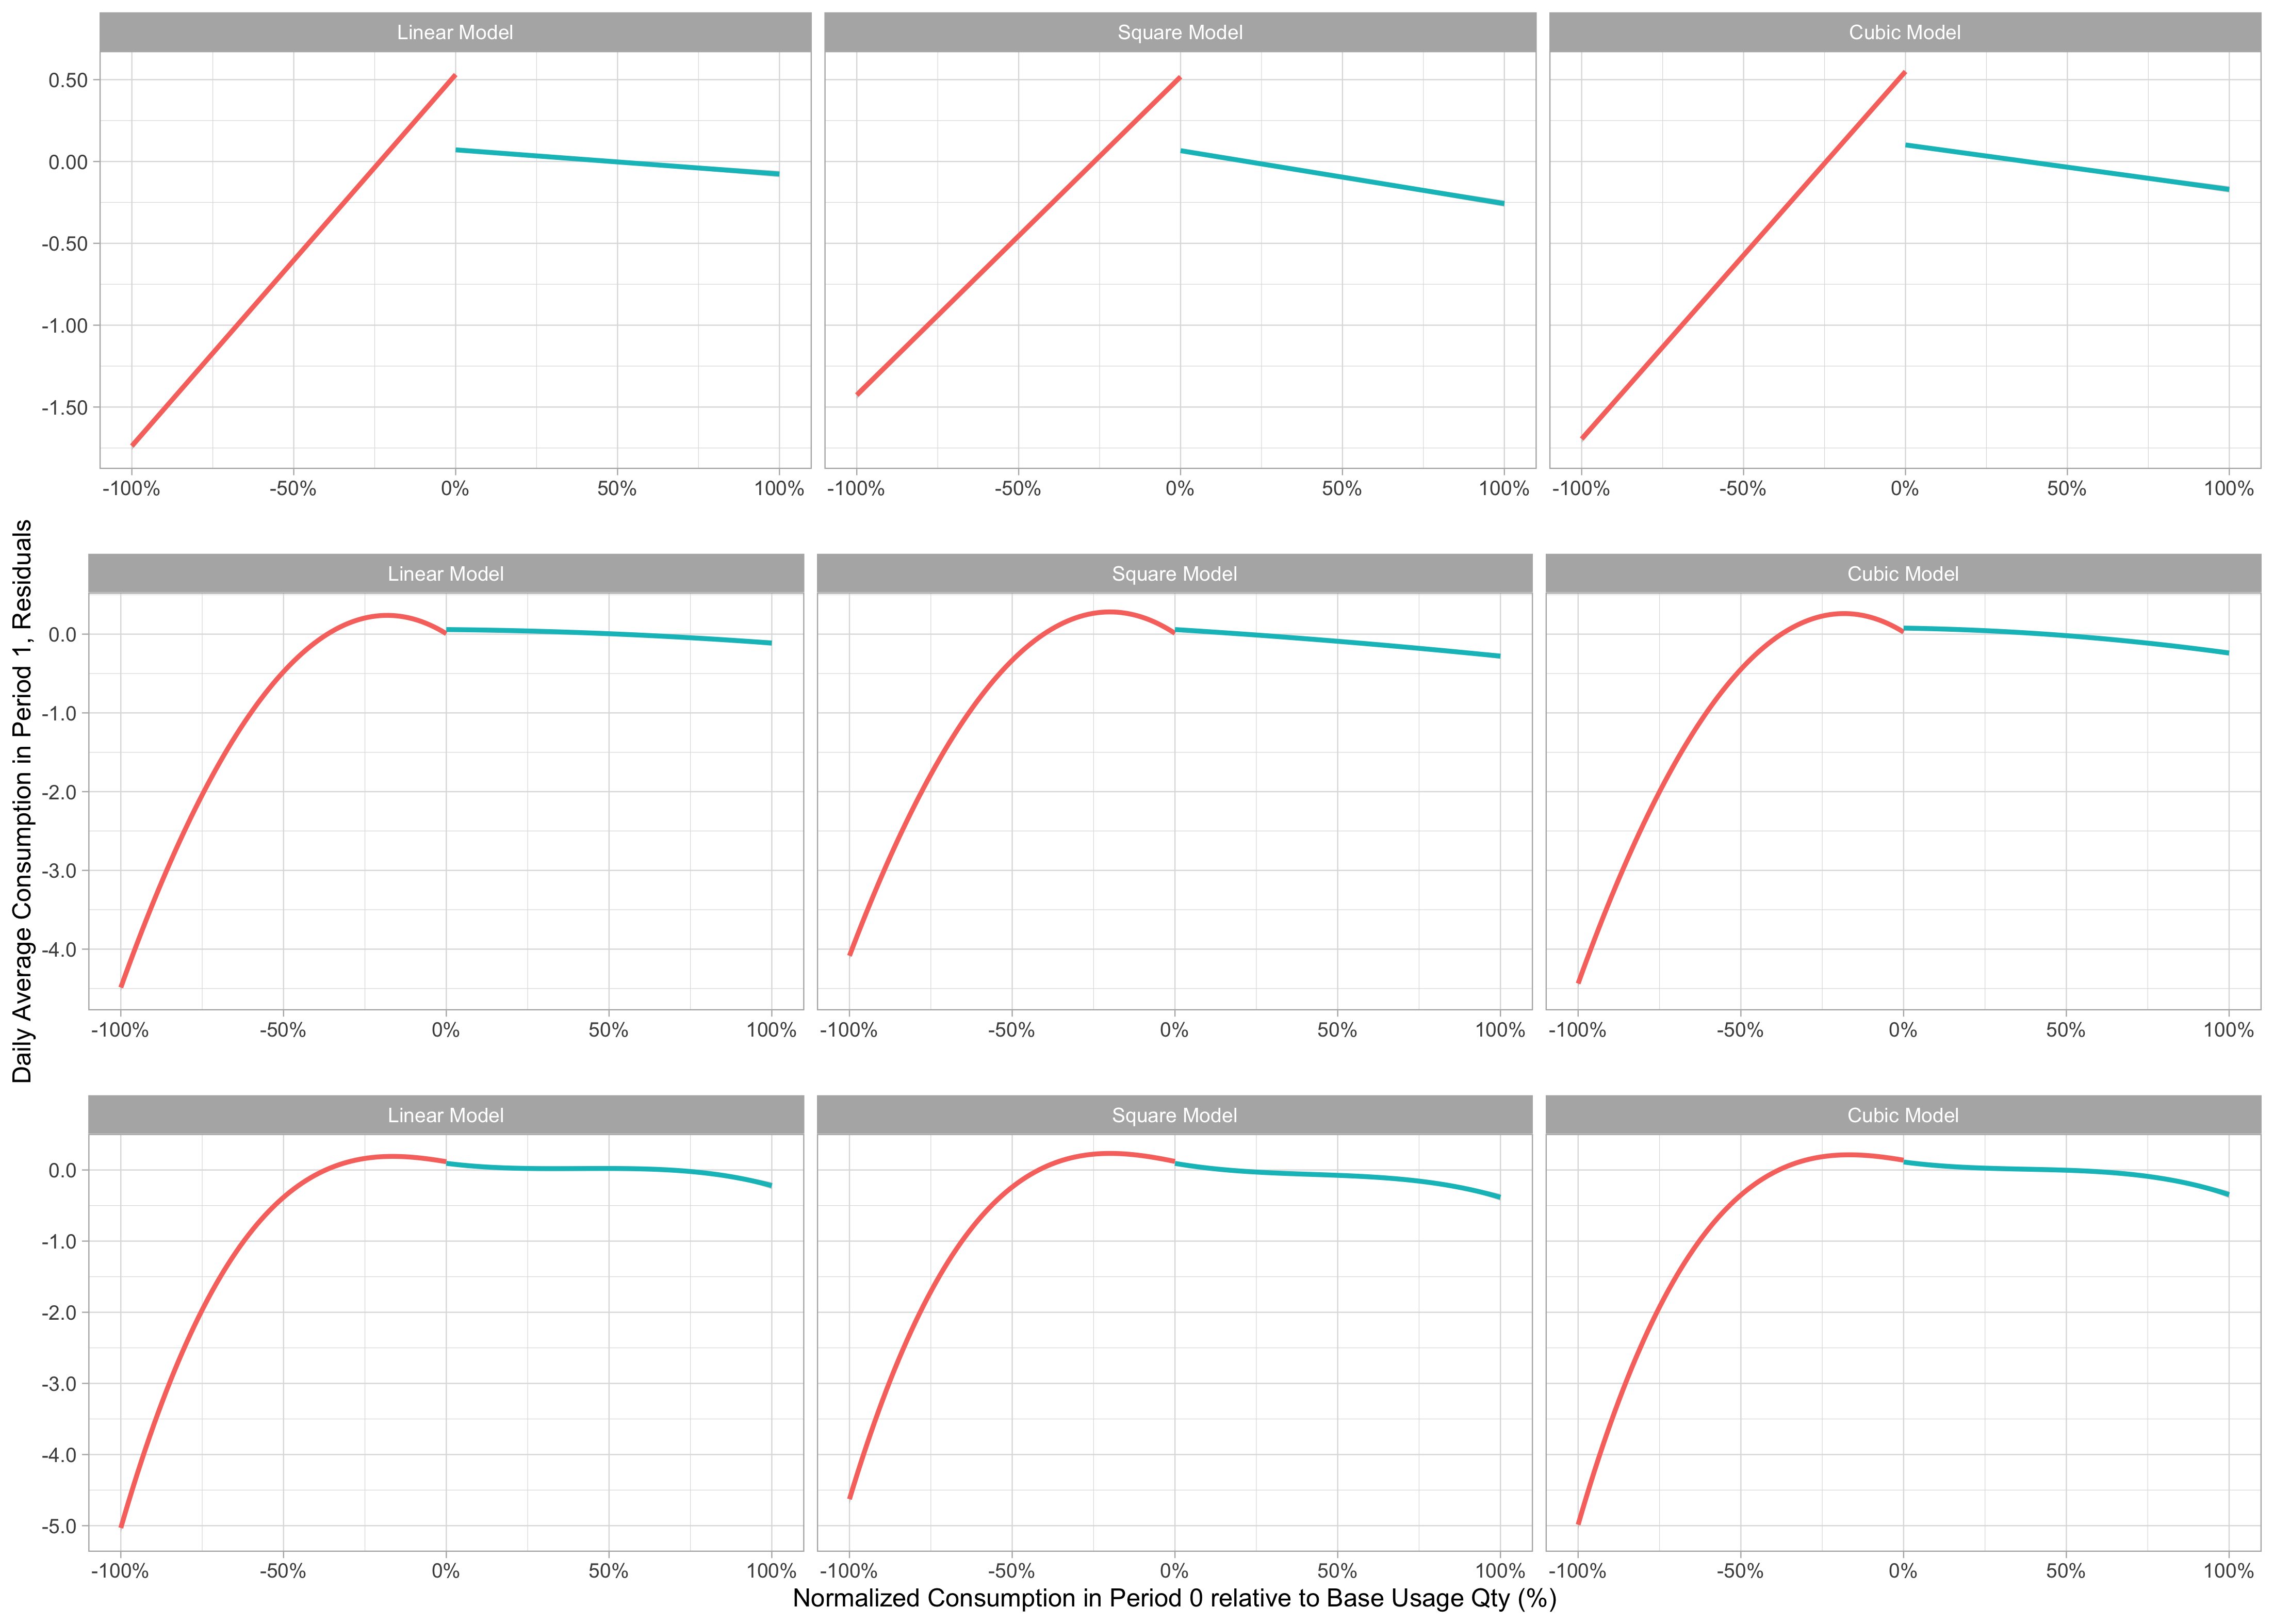
\includegraphics[scale = 0.085]{02_Plots/SMUD-Billing-Data_RD-Approach_Residuals_BW-NA}
    \caption{Spline Fits - By using Residuals}
    \label{Figure:Residuals_NA}
\end{figure}


\end{document}

